\documentclass[utf8x]{beamer}

% This file is a solution template for:

% - Talk at a conference/colloquium.
% - Talk length is about 20min.
% - Style is ornate.

\mode<presentation>
{
  \usetheme{Warsaw}
  % or ...

  %\setbeamercovered{transparent}
  % or whatever (possibly just delete it)
}


\usepackage[english]{babel}
\usepackage{listings}
\usepackage{ulem}
\usepackage{color}
\usepackage{alltt}
\usepackage{tikz}
\usepackage{pgfplots}

\usepackage[utf8x]{inputenc}


\newcommand\redsout[1]{{\color{red}\sout{\hbox{\color{black}{#1}}}}}

% or whatever

% Or whatever. Note that the encoding and the font should match. If T1
% does not look nice, try deleting the line with the fontenc.


\title{The Efficient Handling of Guards in the Design of RPython's Tracing JIT}

\author[David Schneider, Carl Friedrich Bolz]{David Schneider \and \emph{Carl Friedrich Bolz}}
% - Give the names in the same order as the appear in the paper.
% - Use the \inst{?} command only if the authors have different
%   affiliation.

\institute[Heinrich-Heine-Universität Düsseldorf]{
Heinrich-Heine-Universität Düsseldorf, STUPS Group, Germany
}

\date{2012 VMIL, 21st of October, 2012}
% - Either use conference name or its abbreviation.
% - Not really informative to the audience, more for people (including
%   yourself) who are reading the slides online


% If you have a file called "university-logo-filename.xxx", where xxx
% is a graphic format that can be processed by latex or pdflatex,
% resp., then you can add a logo as follows:




% Delete this, if you do not want the table of contents to pop up at
% the beginning of each subsection:
%\AtBeginSubsection[]
%{
%  \begin{frame}<beamer>
%    \frametitle{Outline}
%    \tableofcontents[currentsection,currentsubsection]
%  \end{frame}
%}


% If you wish to uncover everything in a step-wise fashion, uncomment
% the following command:

%\beamerdefaultoverlayspecification{<+->}


\begin{document}

\begin{frame}
  \titlepage
\end{frame}

%\section{Introduction}

\begin{frame}
  \frametitle{Tracing JITs Compile by Observing an Interpreter}
  \begin{itemize}
      \item VM contains both an interpreter and the tracing JIT compiler
      \item JIT works by observing and logging what the interpreter does
      \item for interesting, commonly executed code paths
      \item produces a linear list of operations (trace)
  \end{itemize}
\end{frame}

\begin{frame}
  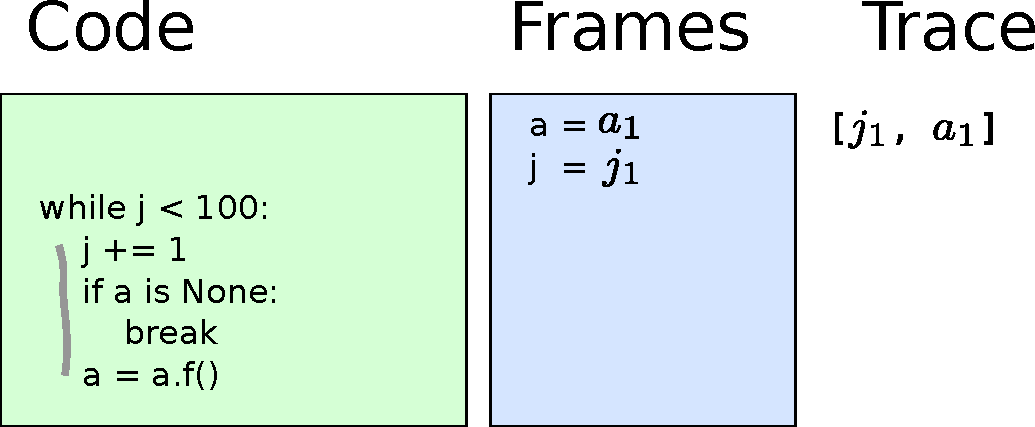
\includegraphics[scale=0.4]{figures/loop01}
\end{frame}

\begin{frame}
  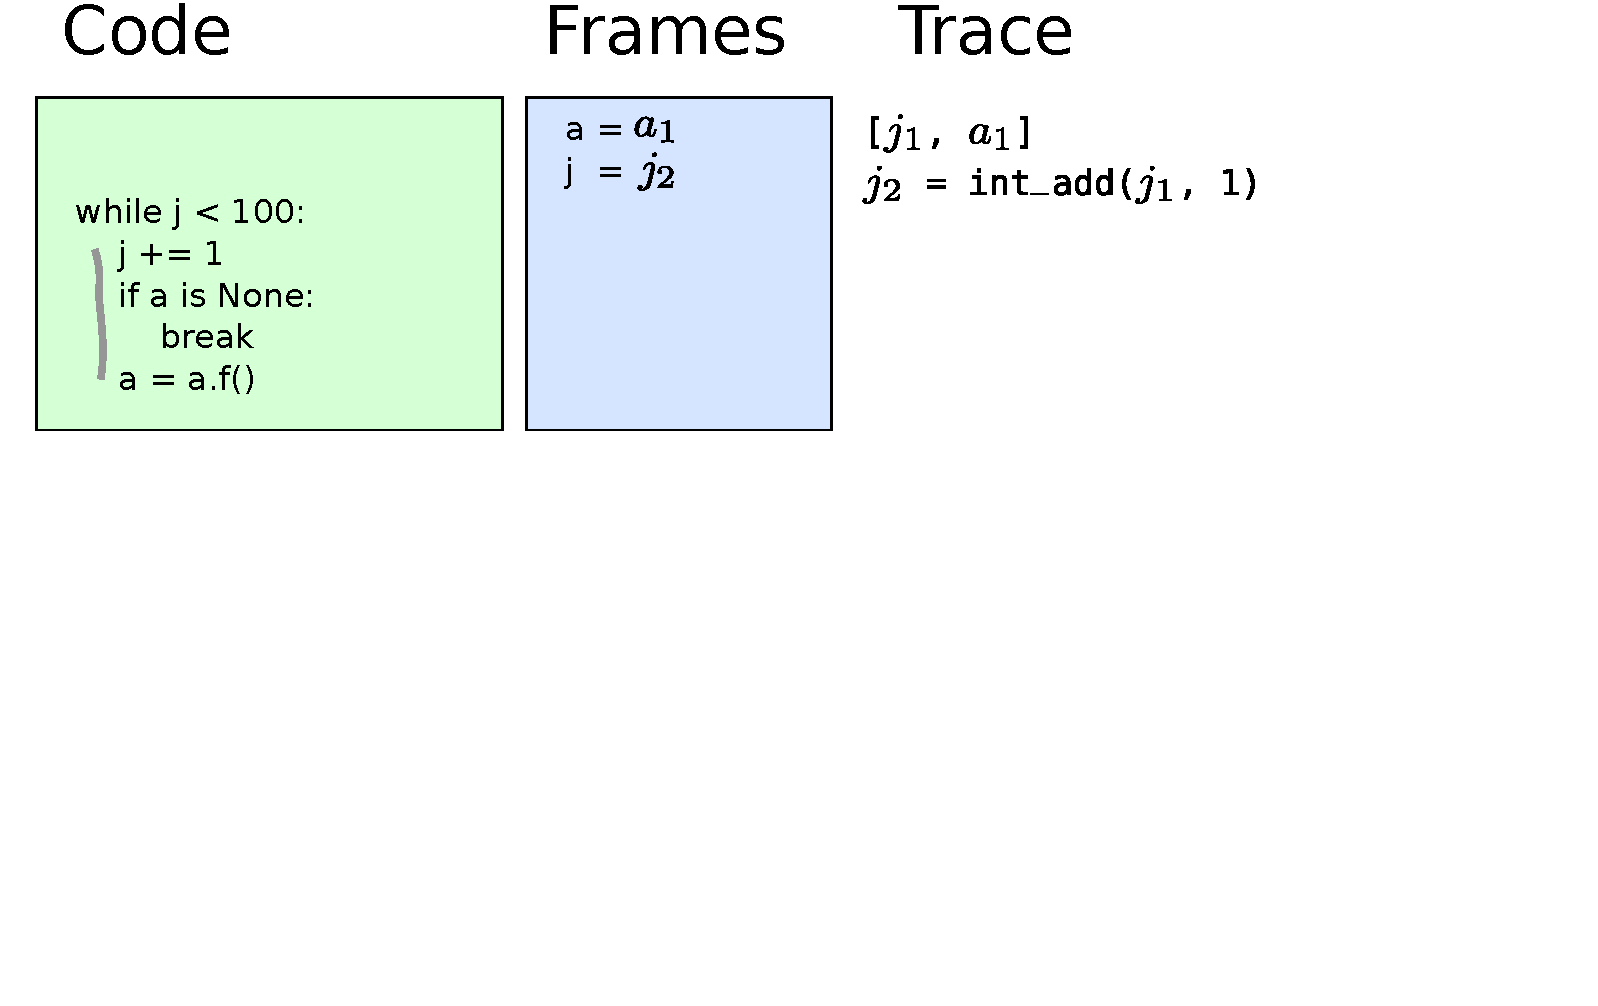
\includegraphics[scale=0.4]{figures/loop02}
\end{frame}

\begin{frame}
  \frametitle{Guards}
  \begin{itemize}
      \item Points of control flow divergence are marked with guards
      \item Operations that check whether conditions are still true
      \item When a guard fails, execution of the trace stops and continues in the interpreter
      \pause
      \item \emph{This talk:} technology and design decisions of guards
      \pause
      \begin{block}{Guard Characteristics}
          \begin{itemize}
              \item lots of them, up to 20\% guards
              \item most never fail
              \item need big information attached to them
          \end{itemize}
      \end{block}
  \end{itemize}
\end{frame}


\begin{frame}
  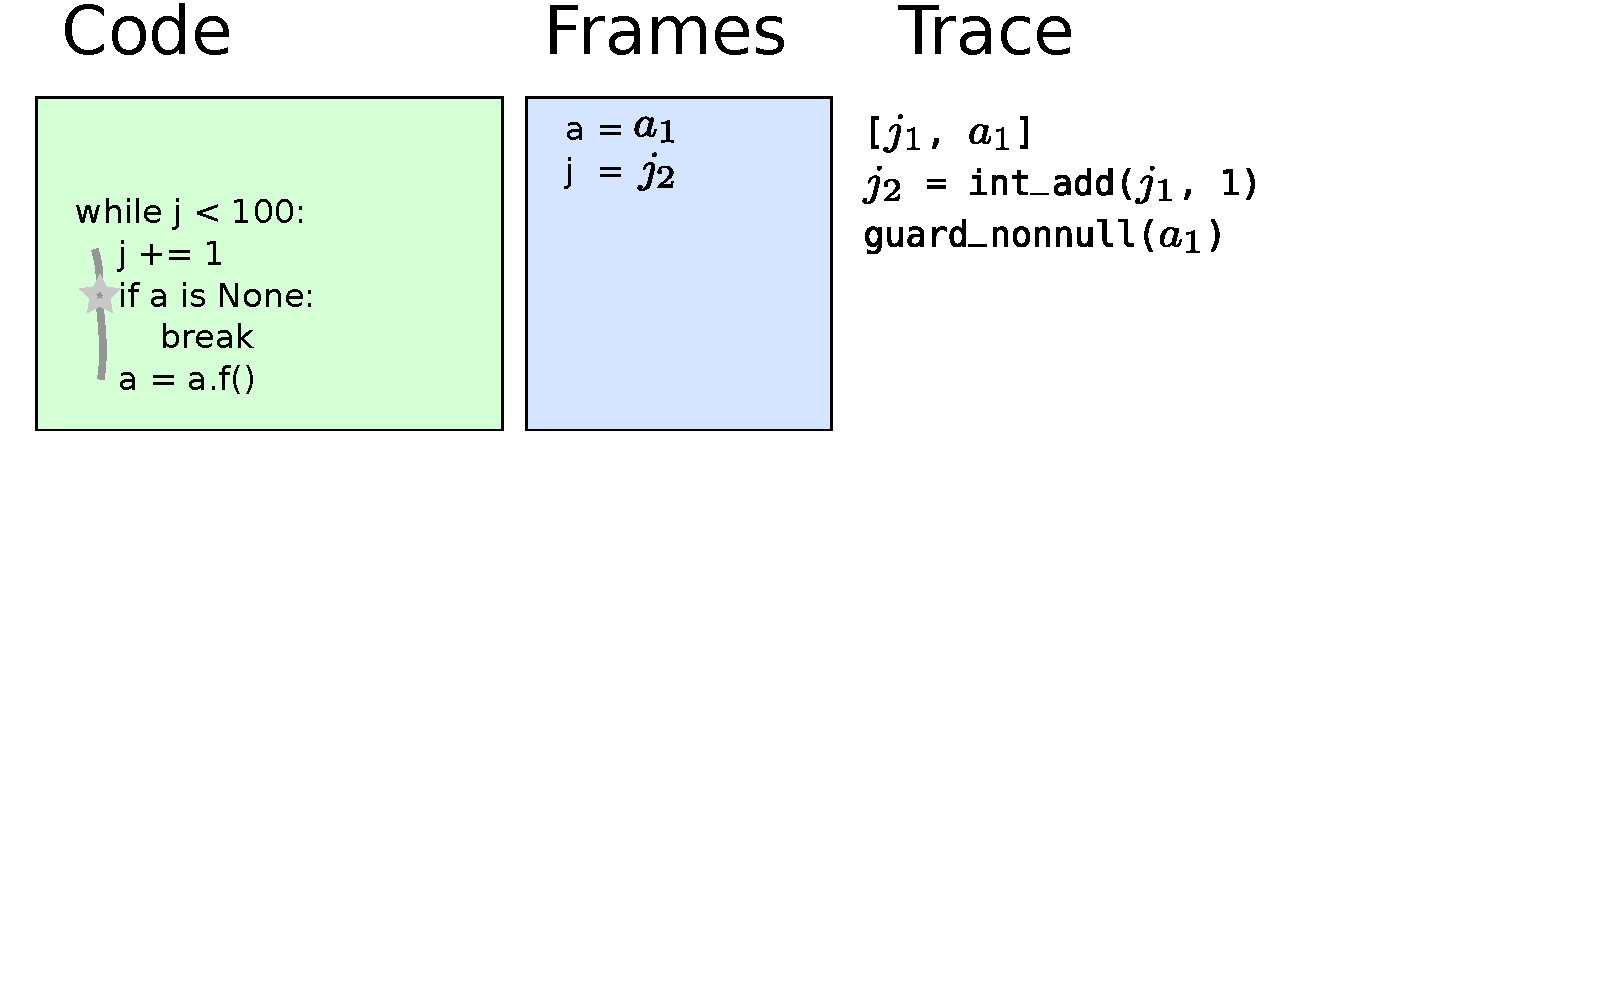
\includegraphics[scale=0.4]{figures/loop03}
\end{frame}

\begin{frame}
  \frametitle{Inlining}
  Tracing automatically does (potentially deep) inlining
\end{frame}


\begin{frame}
  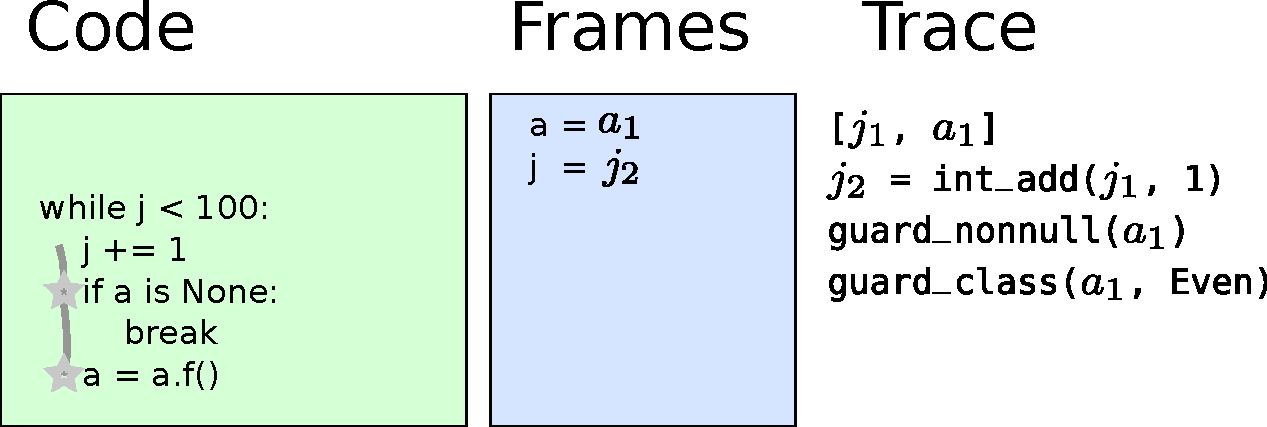
\includegraphics[scale=0.4]{figures/loop04}
\end{frame}

\begin{frame}
  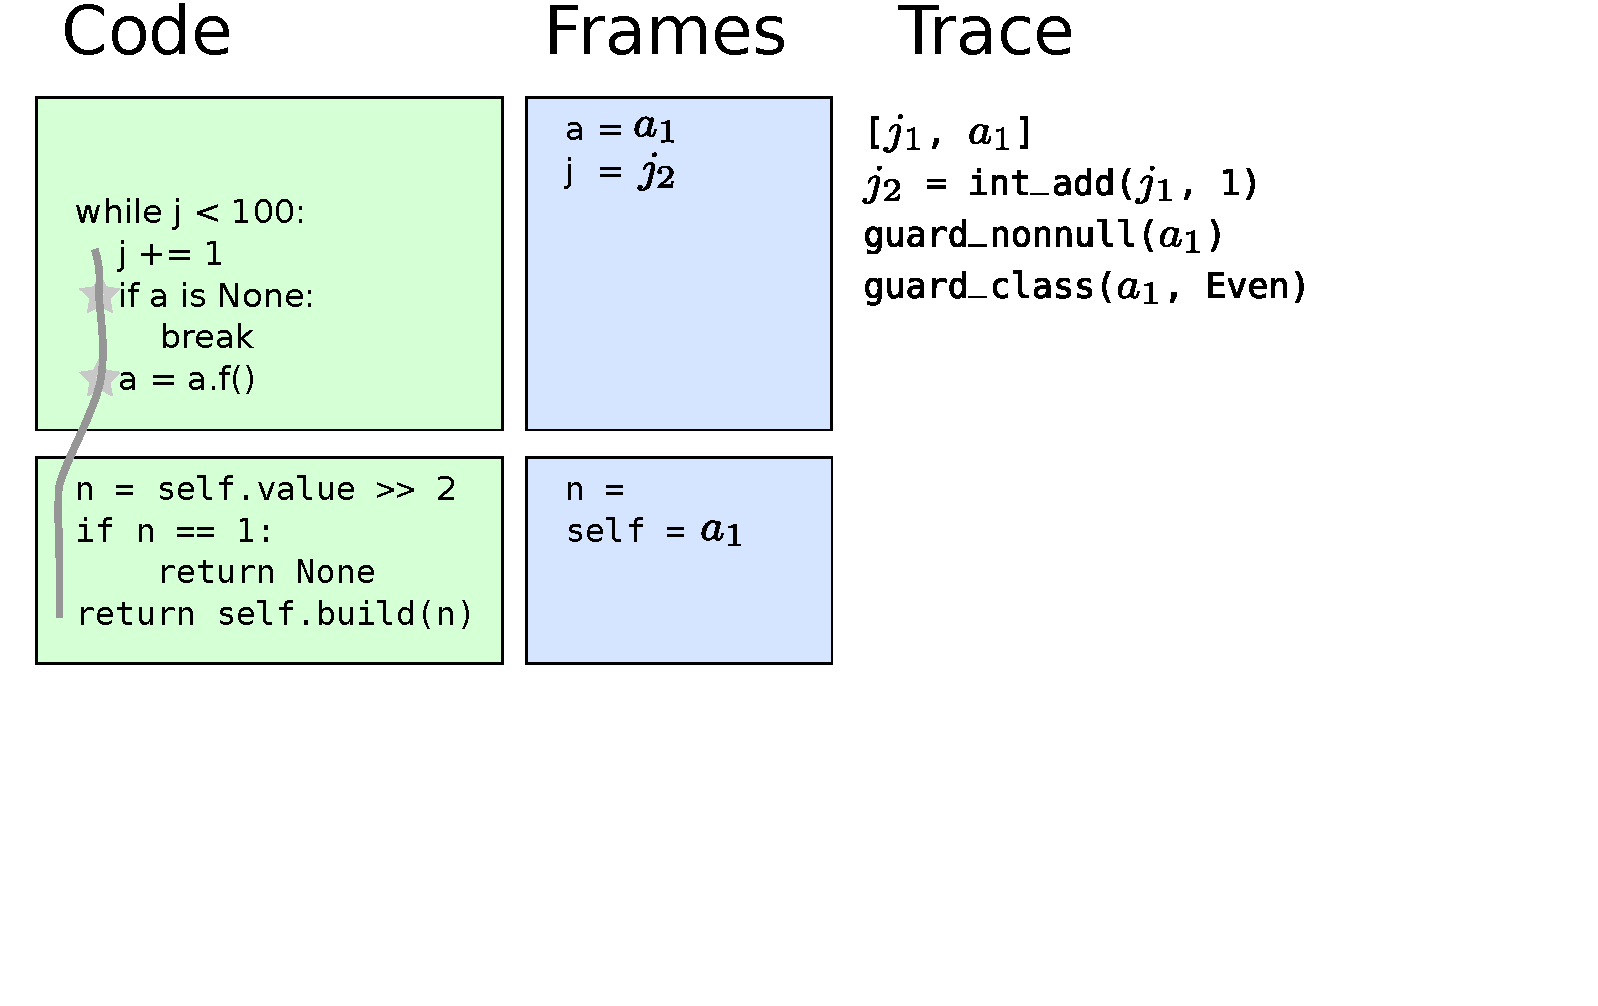
\includegraphics[scale=0.4]{figures/loop05}
\end{frame}

\begin{frame}
  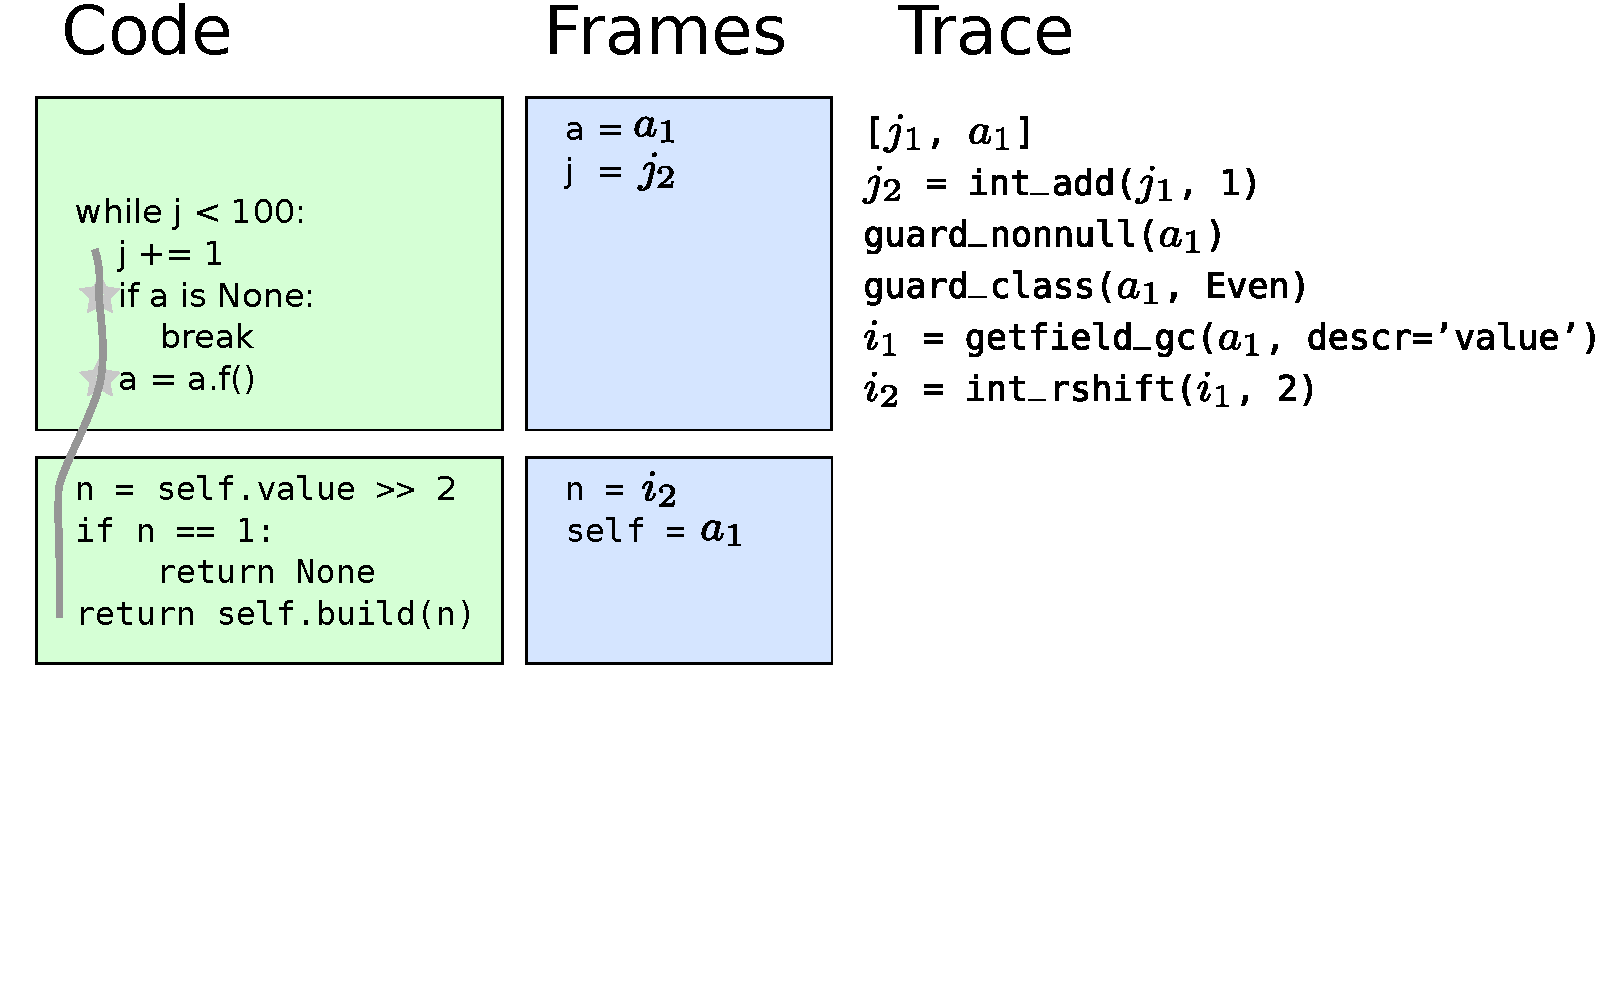
\includegraphics[scale=0.4]{figures/loop06}
\end{frame}

\begin{frame}
  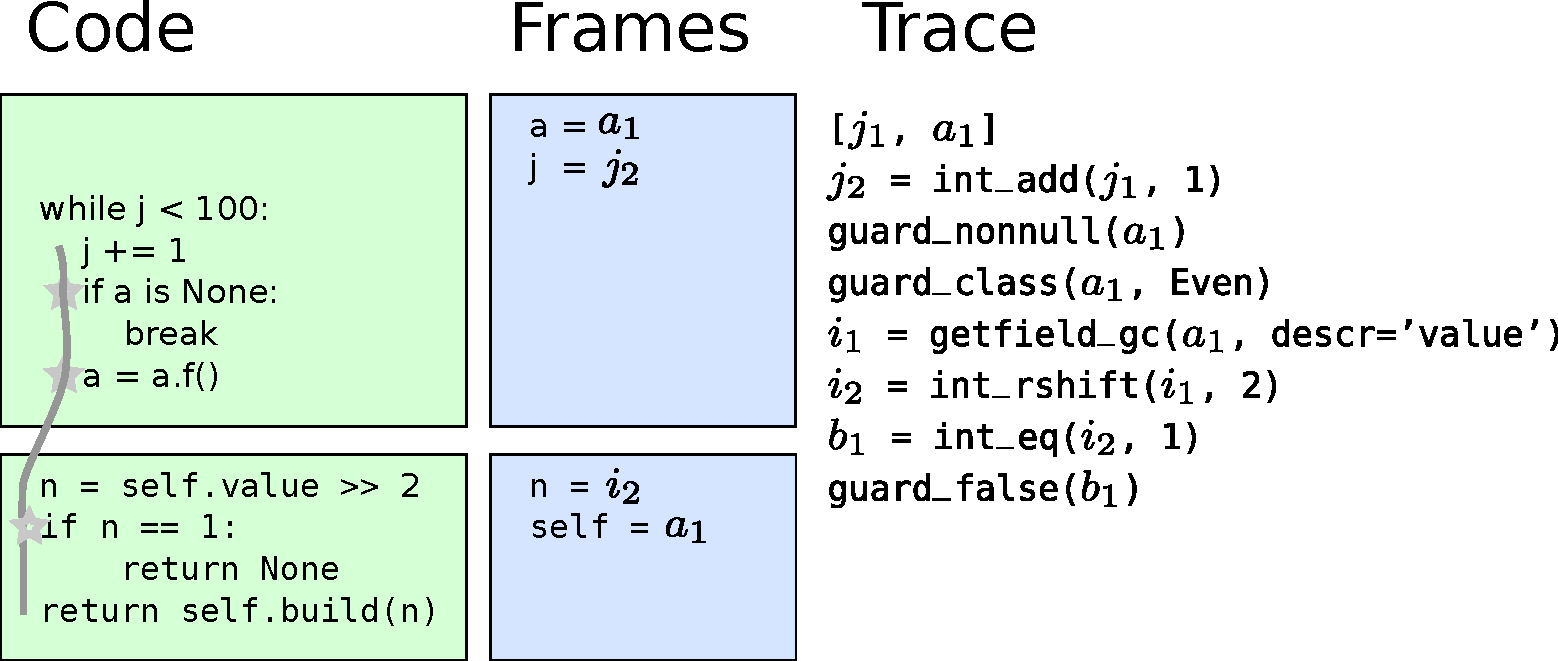
\includegraphics[scale=0.4]{figures/loop07}
\end{frame}

\begin{frame}
  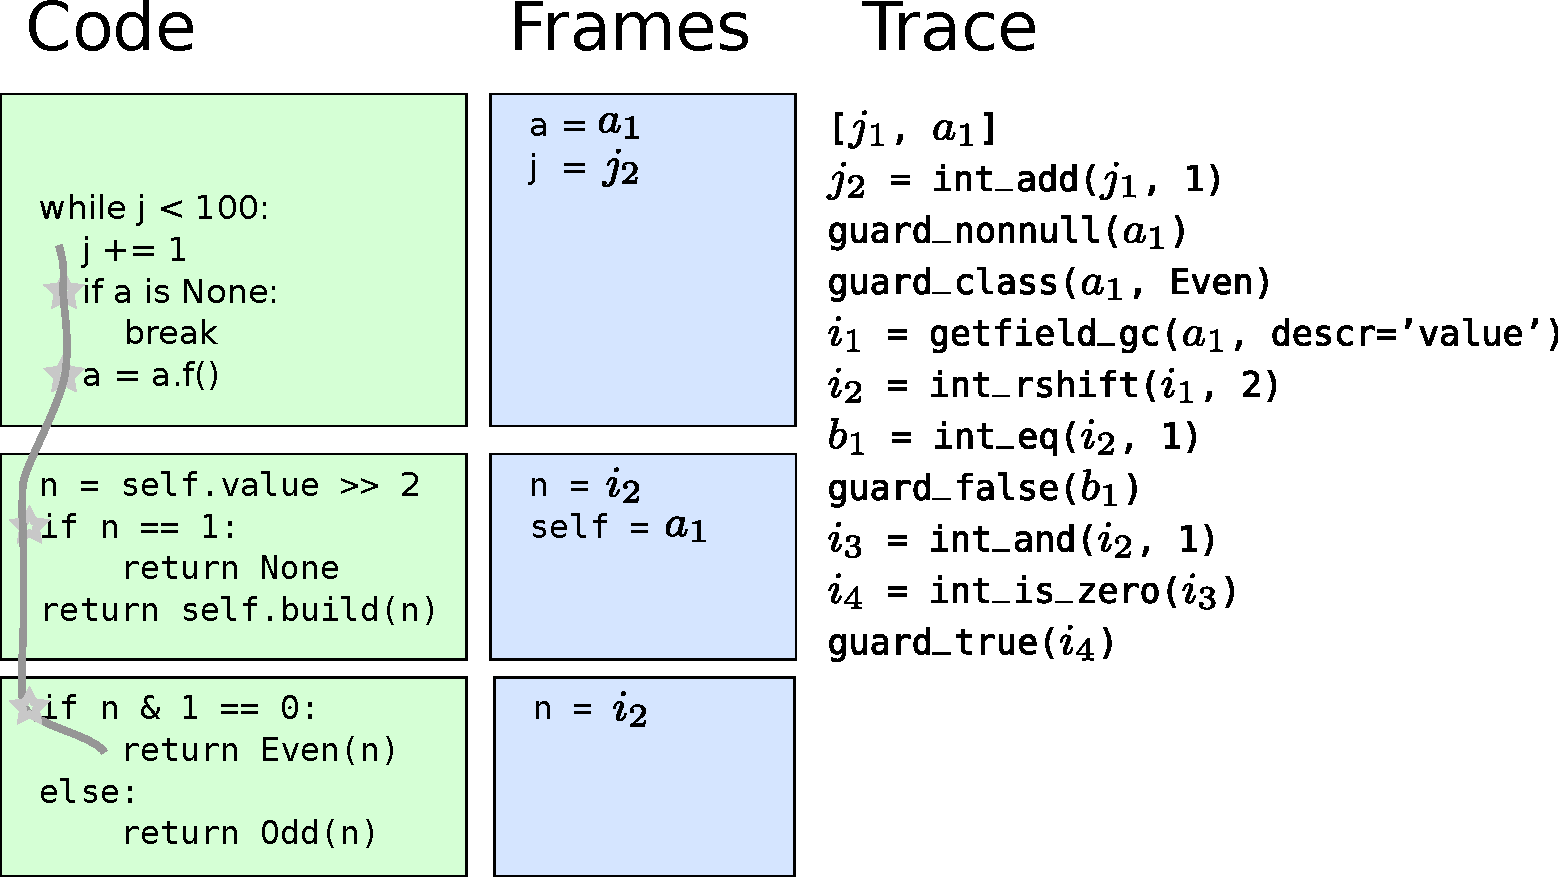
\includegraphics[scale=0.4]{figures/loop08}
\end{frame}

\begin{frame}
  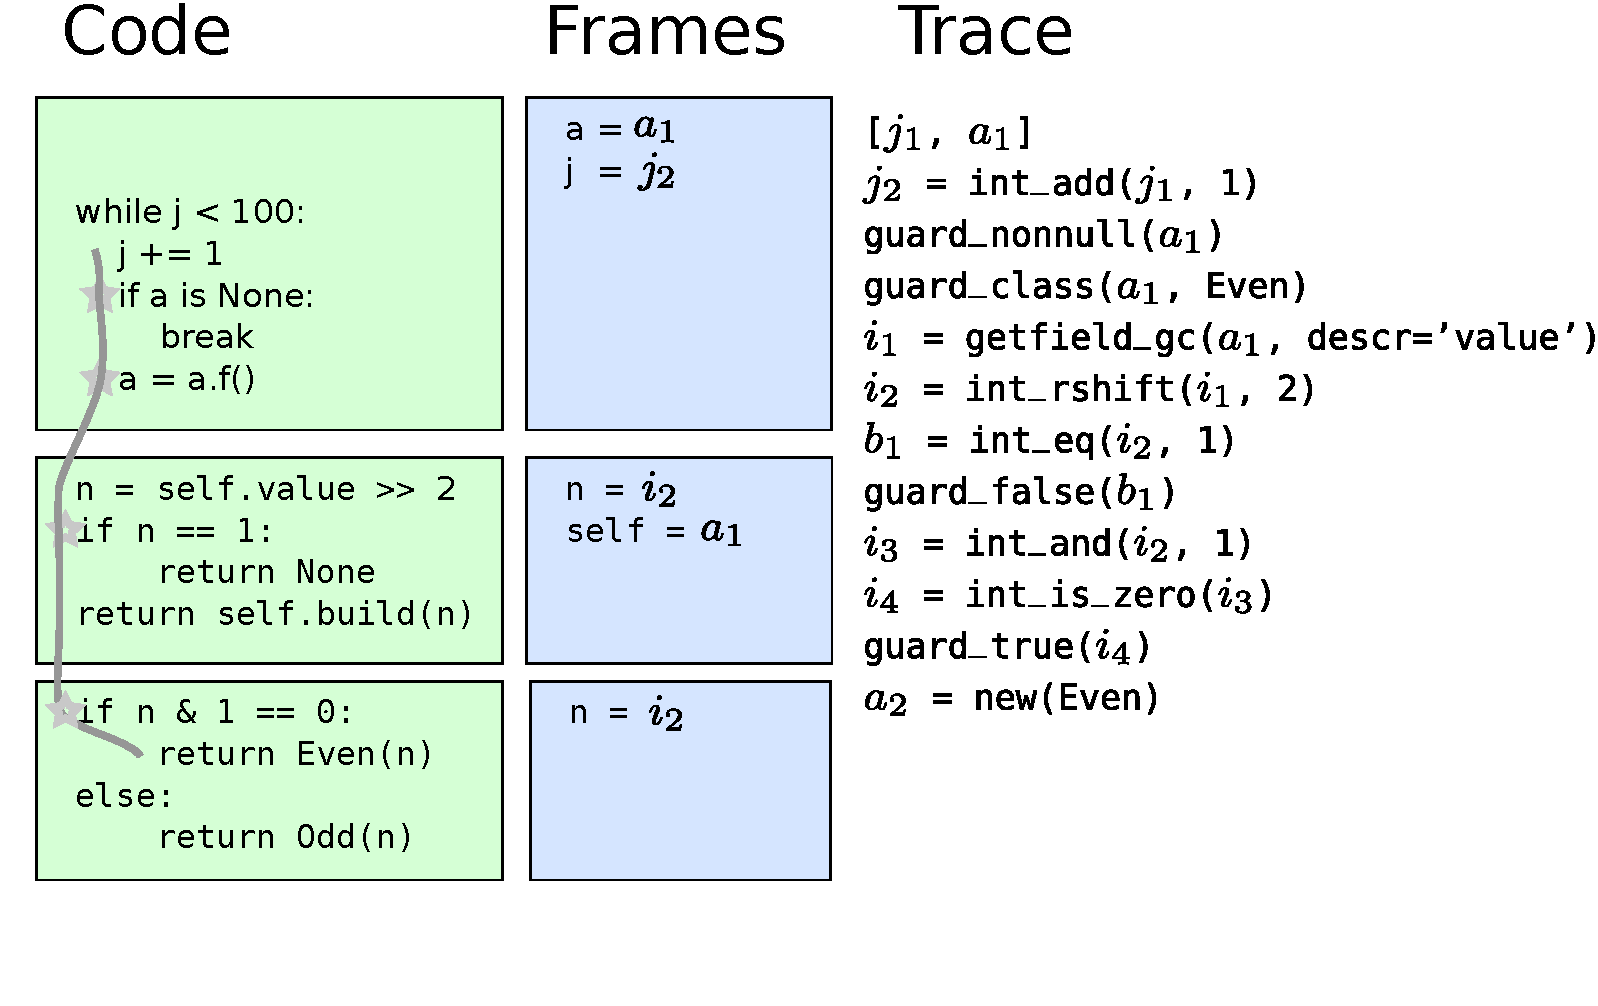
\includegraphics[scale=0.4]{figures/loop09}
\end{frame}

\begin{frame}
  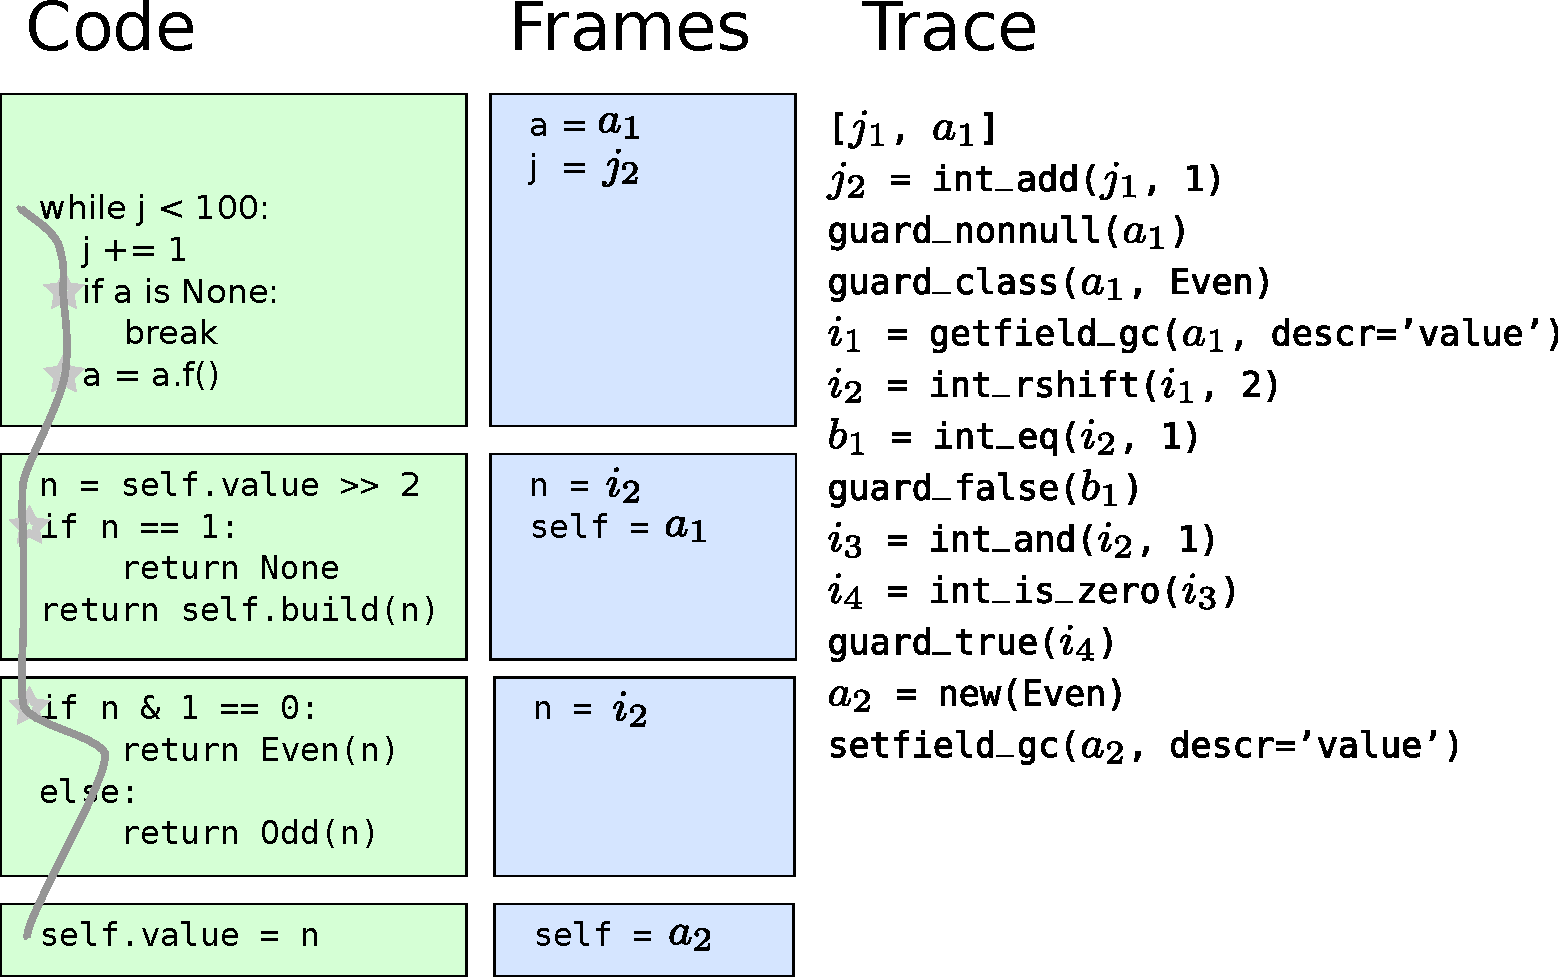
\includegraphics[scale=0.4]{figures/loop10}
\end{frame}

\begin{frame}
  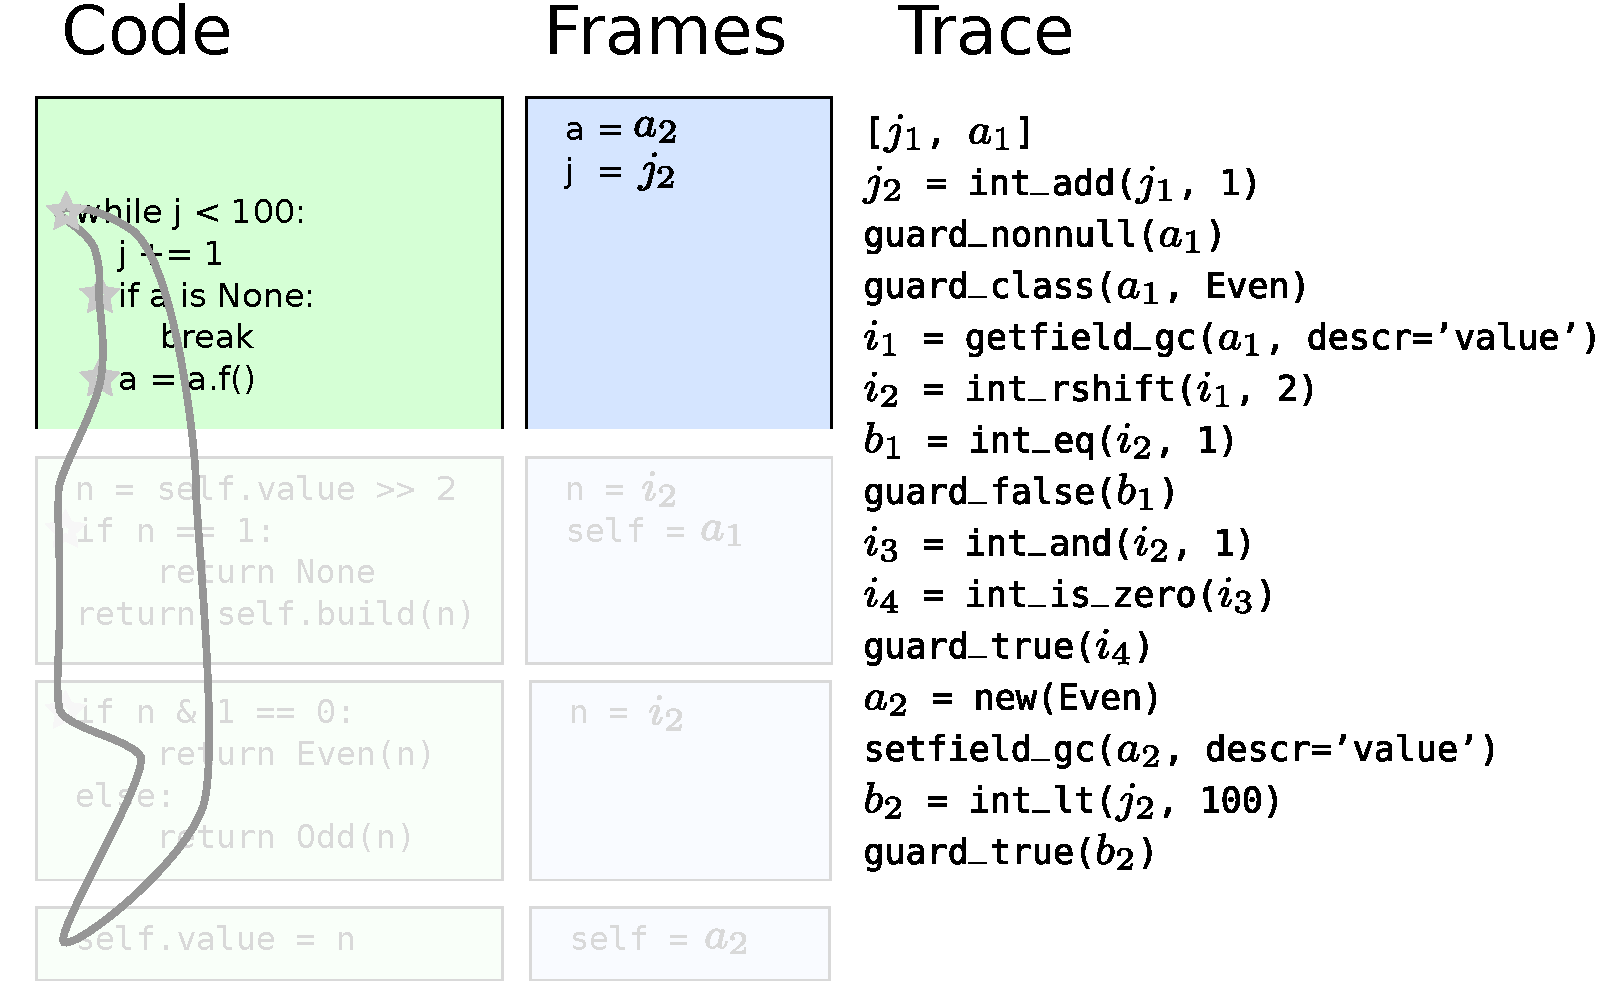
\includegraphics[scale=0.4]{figures/loop11}
\end{frame}

\begin{frame}
  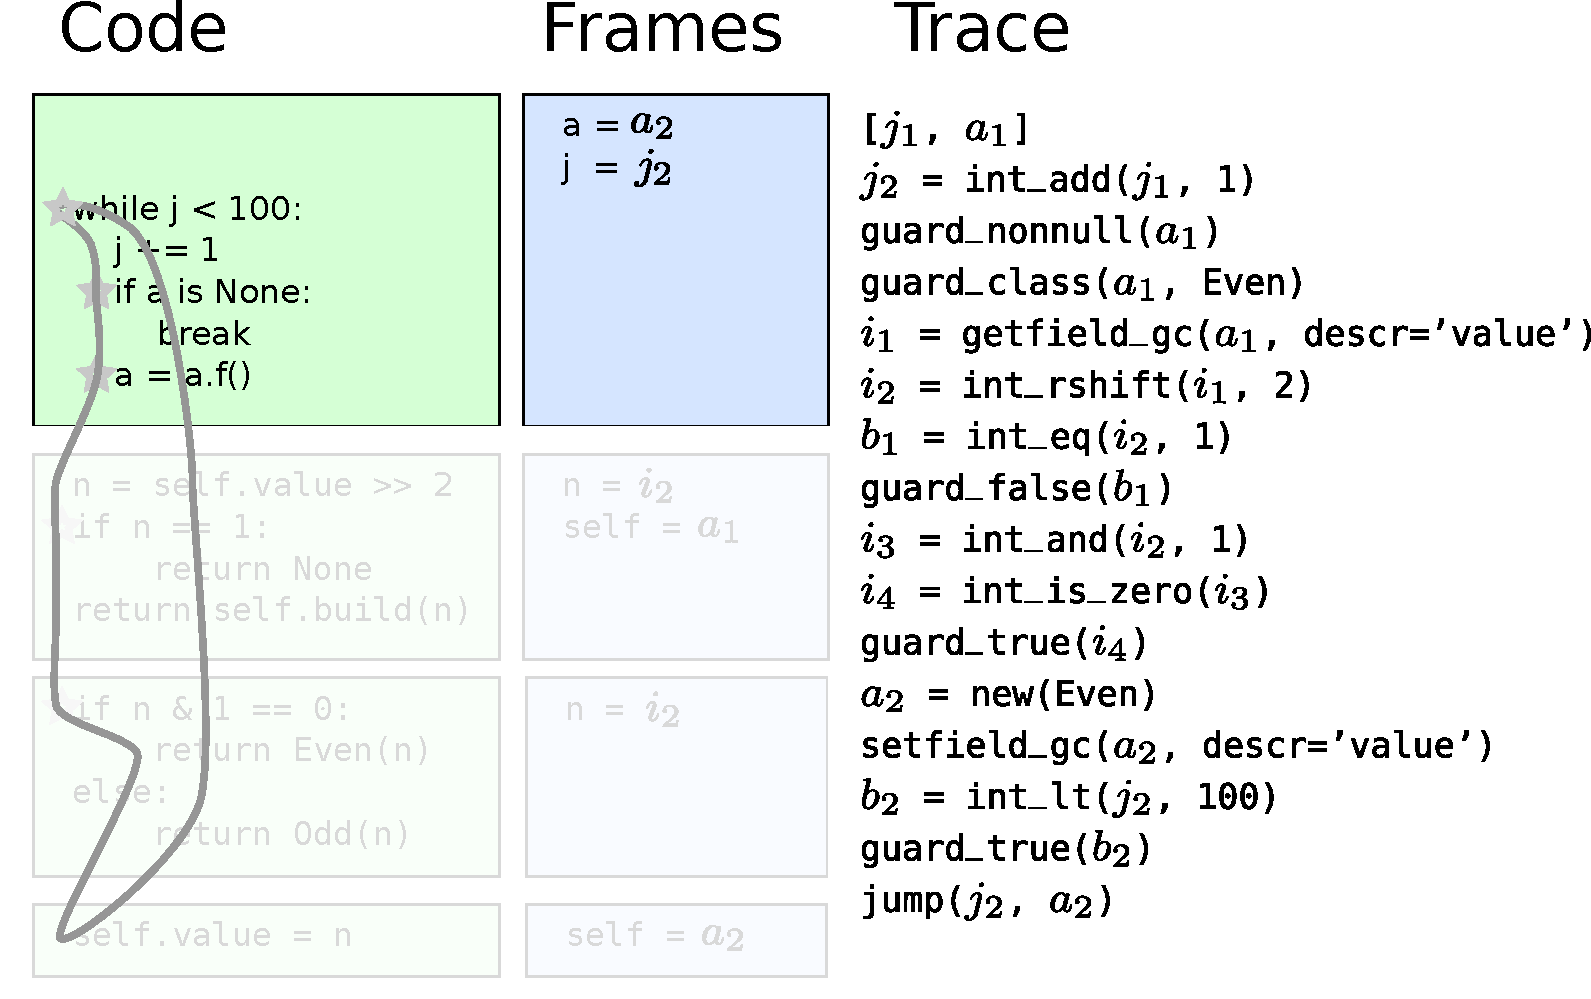
\includegraphics[scale=0.4]{figures/loop12}
\end{frame}

% this talk wants to go over a lot of details that are usually glossed over as
% "easy" when tracing JITs are introduced.

\begin{frame}
  \frametitle{Bridges}
  \begin{itemize}
      \item When a trace fails often, it becomes worth to attach a new trace to it
          \item This is called a bridge
          \item The bridge is attached by patching the guard machine code
          \item when this guard fails in the future, the new trace is executed instead
  \end{itemize}
\end{frame}

\begin{frame}
  \frametitle{RPython and PyPy}
  \begin{itemize}
      \item Context: RPython
      \item a generic tracing JIT, applicable to many languages
      \item main use: PyPy, an efficient Python interpreter
  \end{itemize}
\end{frame}

%\section{High-Level}

\begin{frame}
  \frametitle{Symbolic Frame Capturing}
  \begin{itemize}
      \item Guard can fail deep inside inlined function
      \item when going back to the interpreter, call stack needs to be re-created
      \item done with the help of symbolic frame stacks
      \item these show how trace variables fill the to-be-built stack frames
  \end{itemize}
\end{frame}

\begin{frame}
  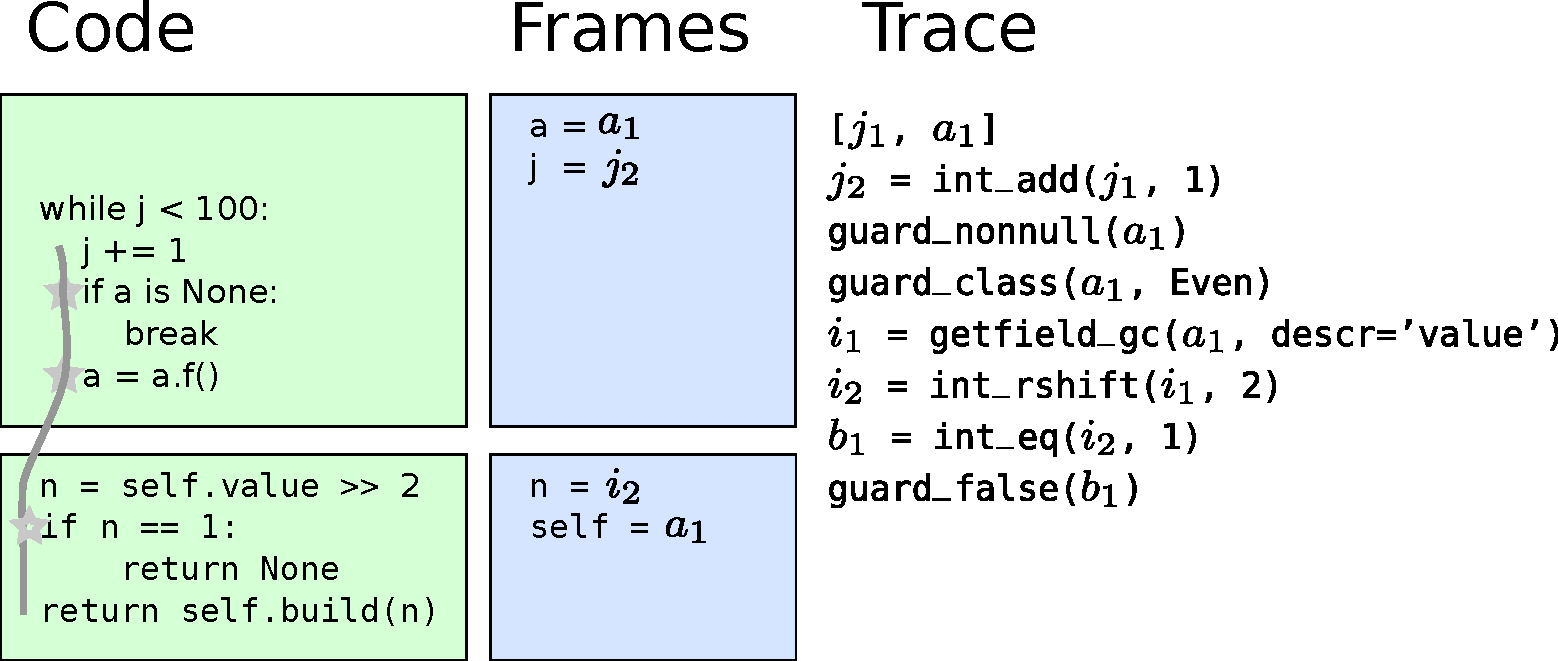
\includegraphics[scale=0.4]{figures/loop07}
\end{frame}

\begin{frame}
  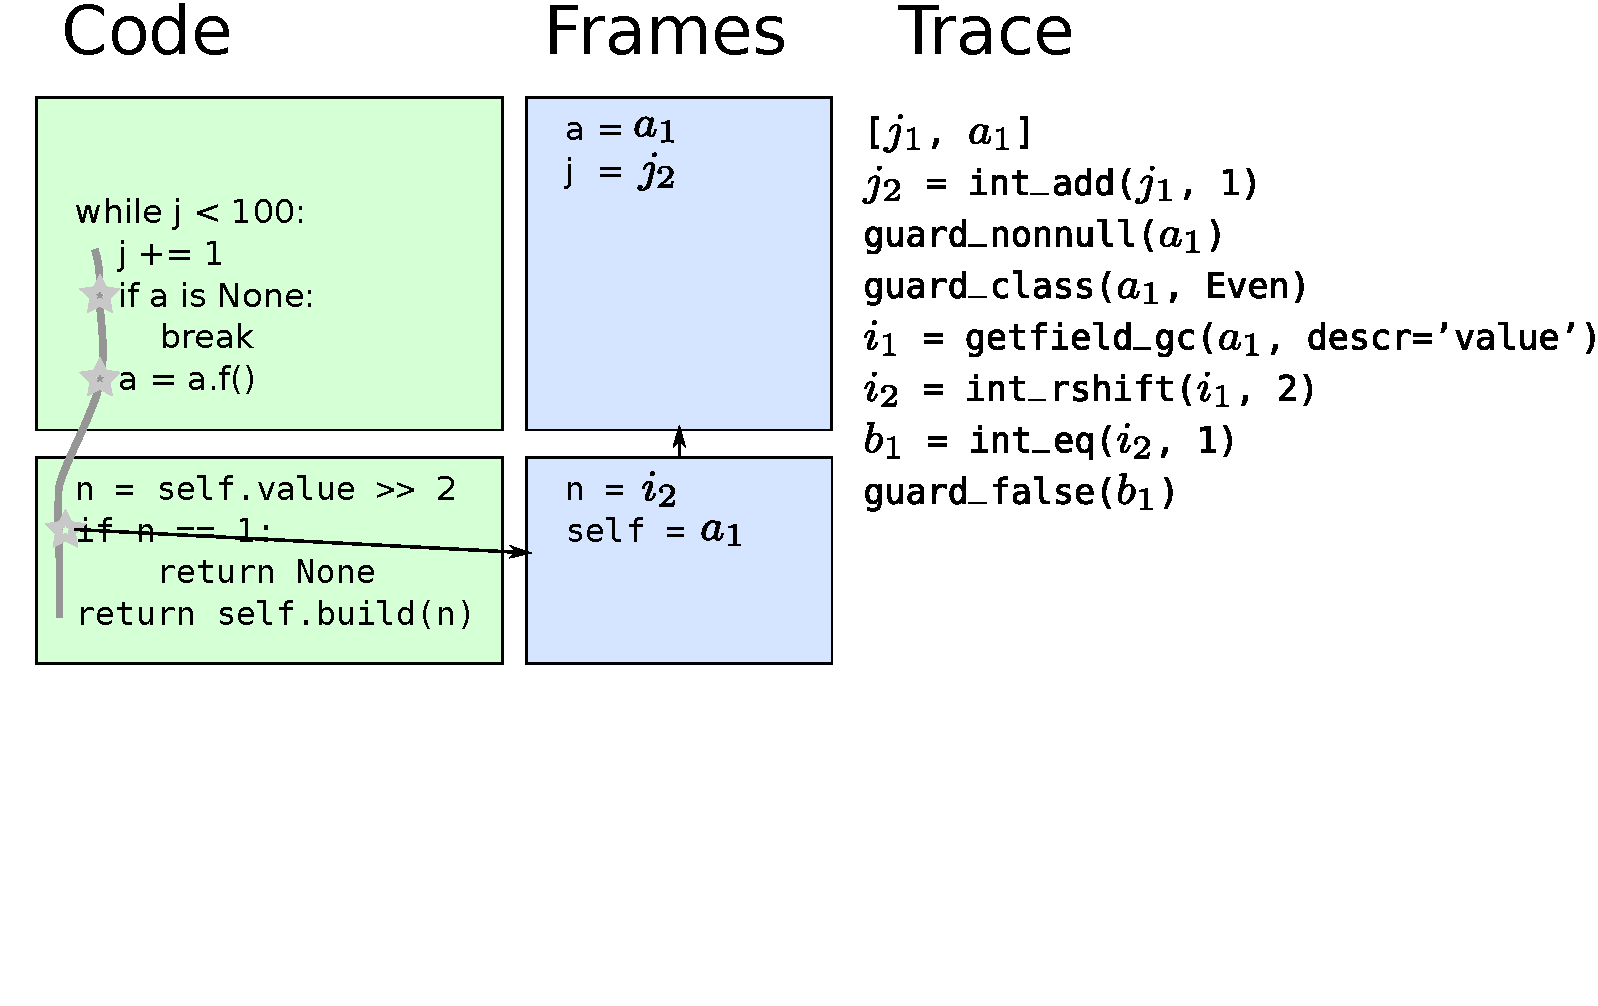
\includegraphics[scale=0.4]{figures/framechain1}
\end{frame}


\begin{frame}
  \frametitle{Symbolic Frame Compression}
  \begin{itemize}
      \item There are \emph{a lot of} guards
      \item Naively storing symbolic frames would be costly in terms of memory
      \item need to store them compactly
      \item observation: from one guard to the next, the non-top stack frames don't change
      \item share these between subsequent guards
      \pause
      \item also need a byte-saving binary representation, but that's just boring work
  \end{itemize}
\end{frame}

\begin{frame}
  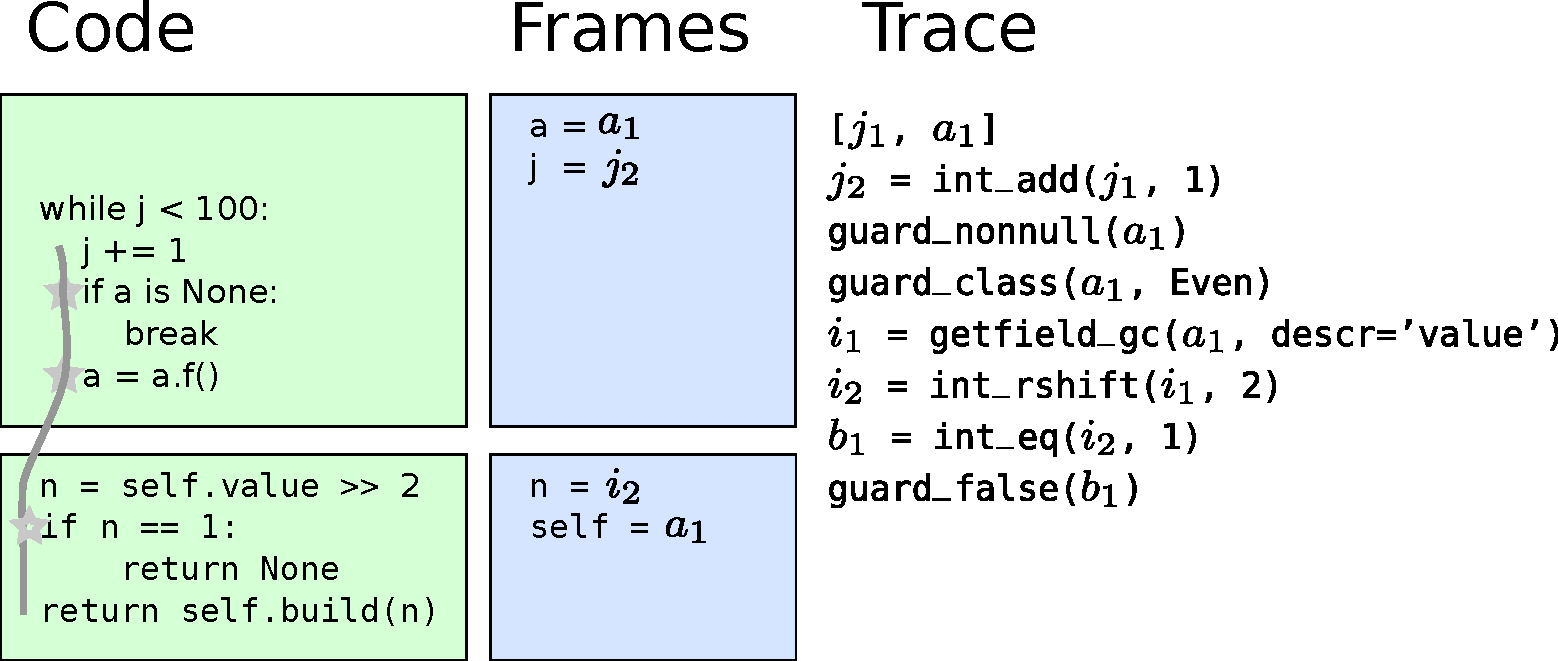
\includegraphics[scale=0.4]{figures/loop07}
\end{frame}

\begin{frame}
  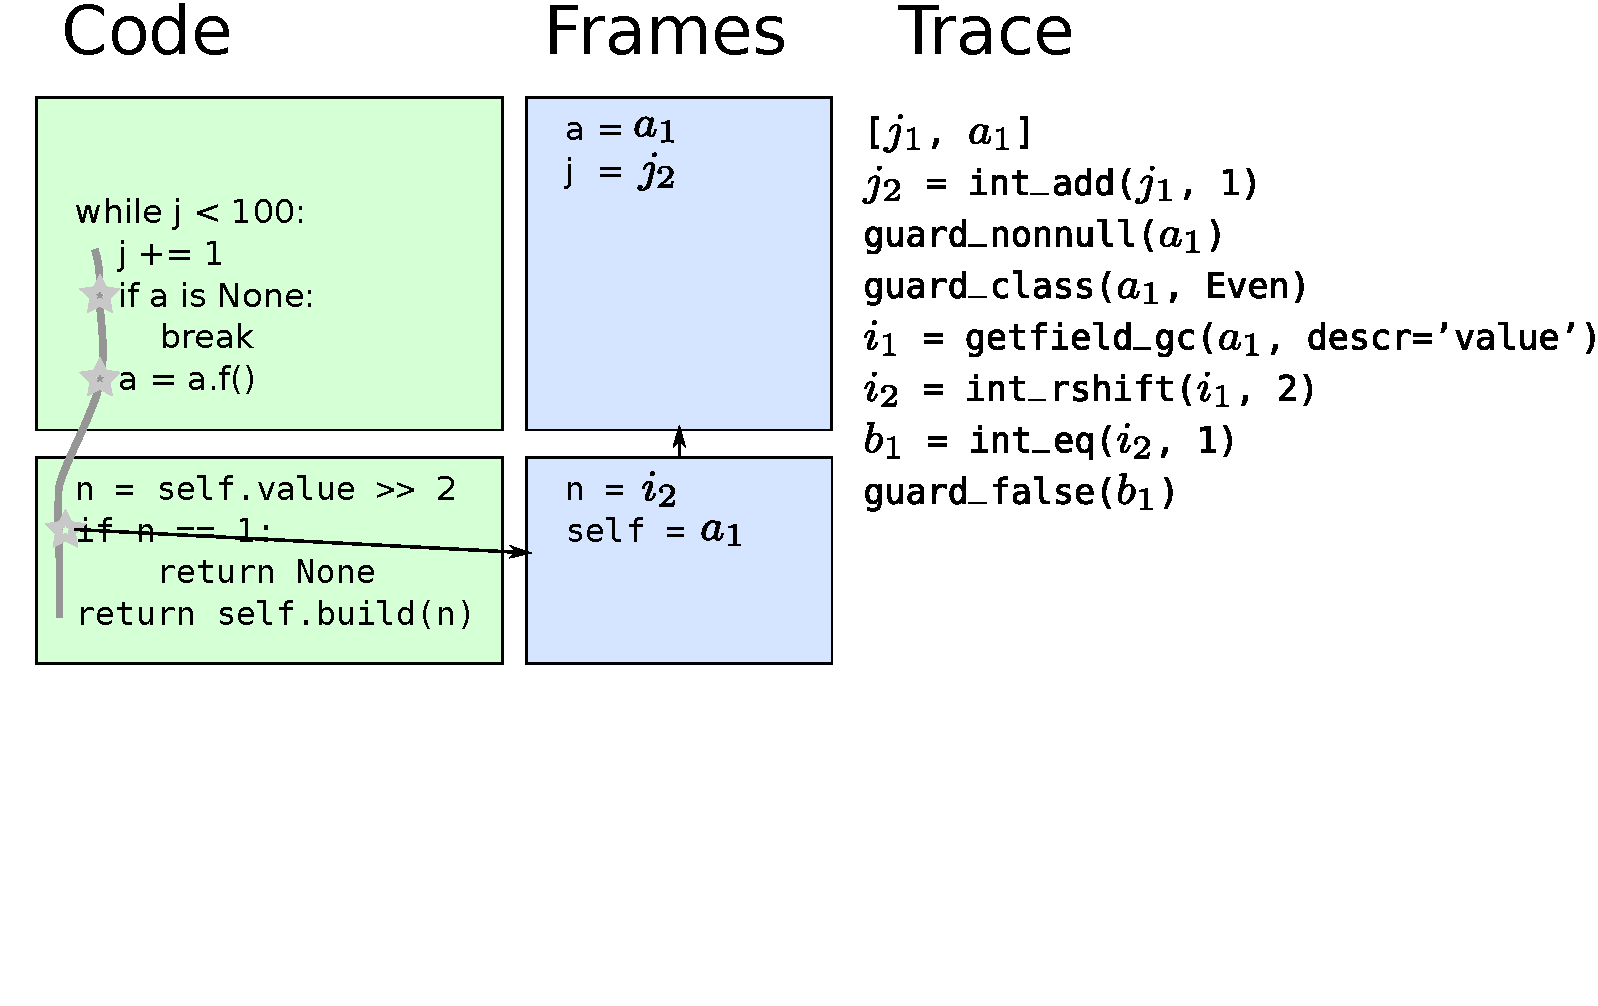
\includegraphics[scale=0.4]{figures/framechain1}
\end{frame}

\begin{frame}
  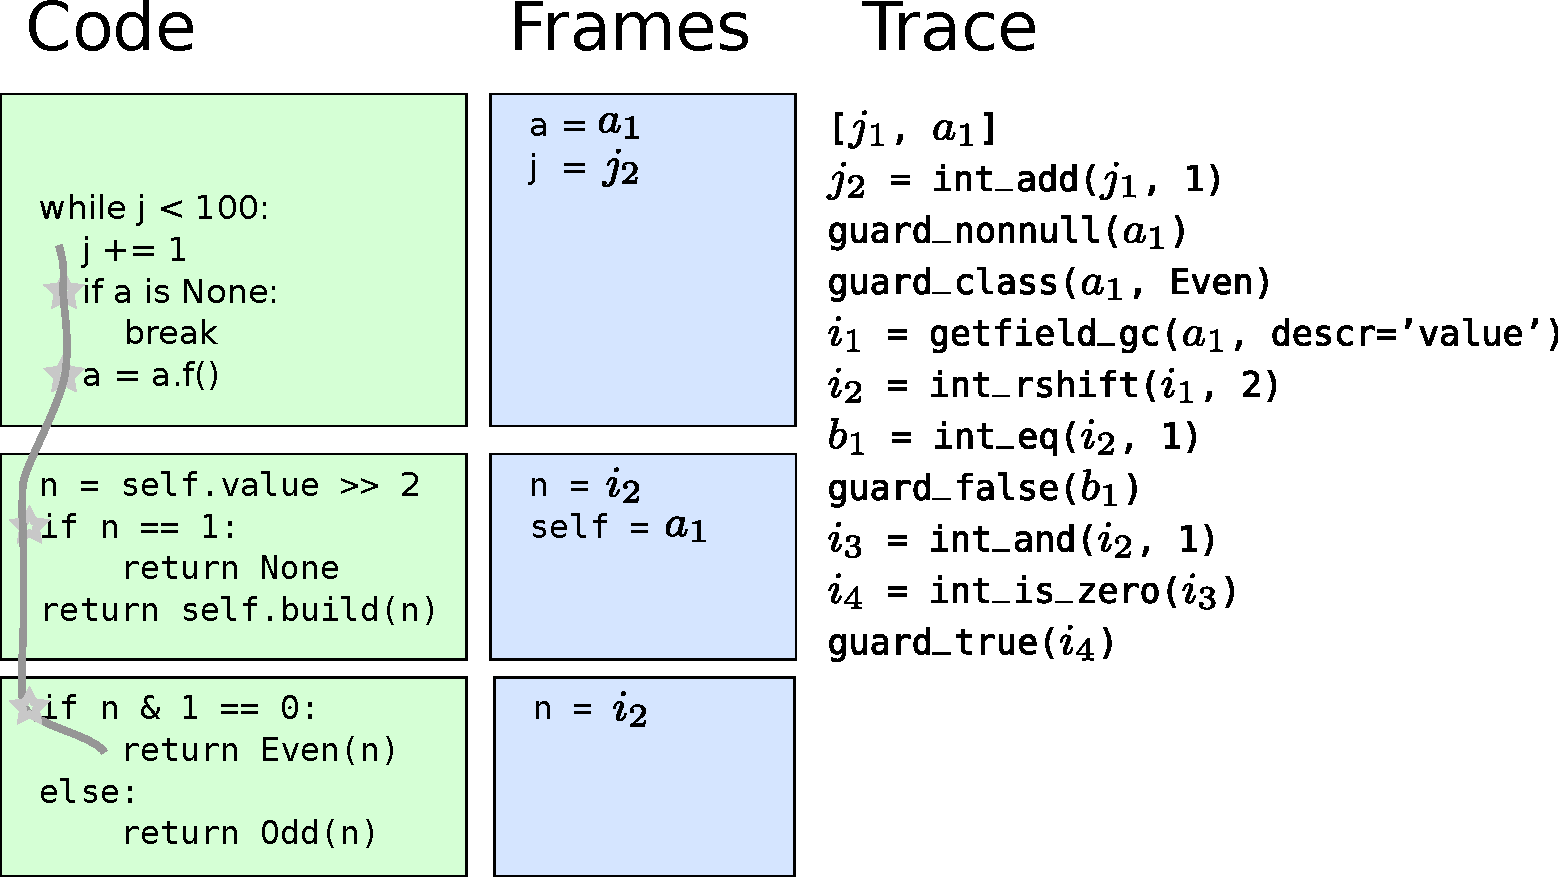
\includegraphics[scale=0.4]{figures/loop08}
\end{frame}

\begin{frame}
  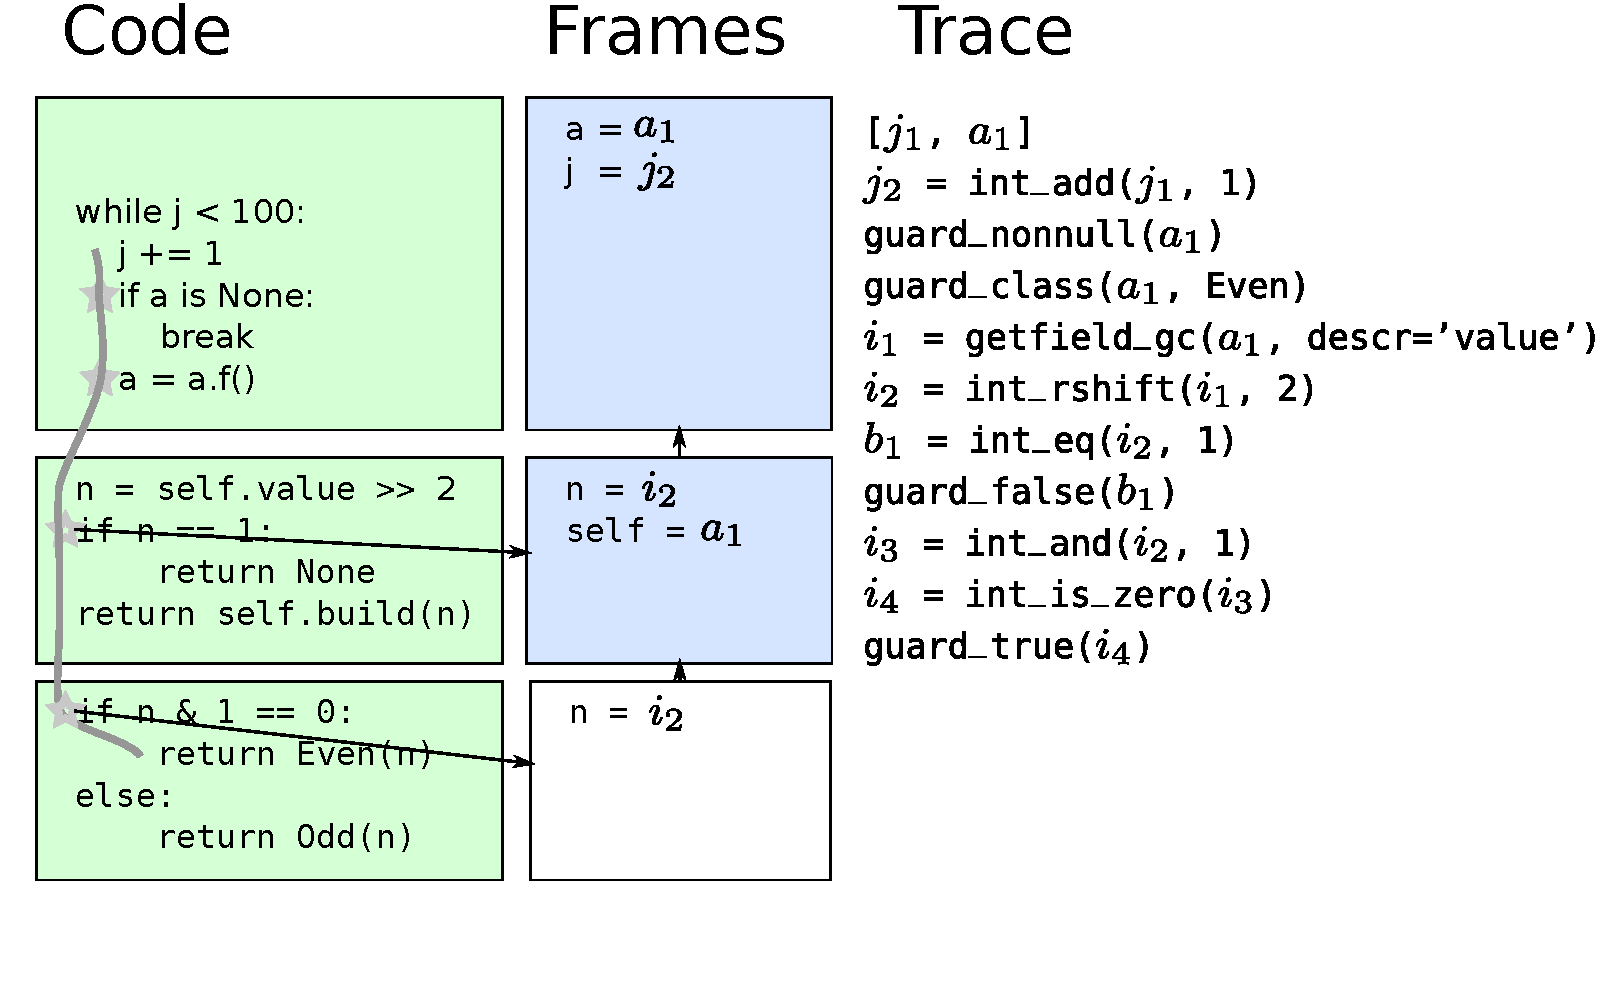
\includegraphics[scale=0.4]{figures/framechain2}
\end{frame}

\begin{frame}
  \frametitle{Interaction with Optimization}
  \begin{itemize}
      \item Some optimizations make it necessary to store extra information in symbolic frames
      \pause
      \item examples:
          \begin{itemize}
              \item allocation removal (need to allocate objects before resuming)
              \item delayed heap stores (need to do stores before resuming interpreter)
          \end{itemize}
      \item can be compressed using similar techniques
  \end{itemize}
\end{frame}

\begin{frame}
  \frametitle{Emitting Guards}
  Guards are compiled as
  \begin{itemize}
    \item quick Check if the condition holds
    \item and a mapping of machine locations to JIT-variables % indirection using the fail-boxes
  \end{itemize}
  \pause
  In case of failure
  \begin{itemize}
    \item execution jumps to shared compensation code, decodes and stores mapping
    \item returns to interpreter that rebuilds state
  \end{itemize}
\end{frame}

\begin{frame}
  \frametitle{Compiling a Trace}
  \begin{figure}
  \centering
  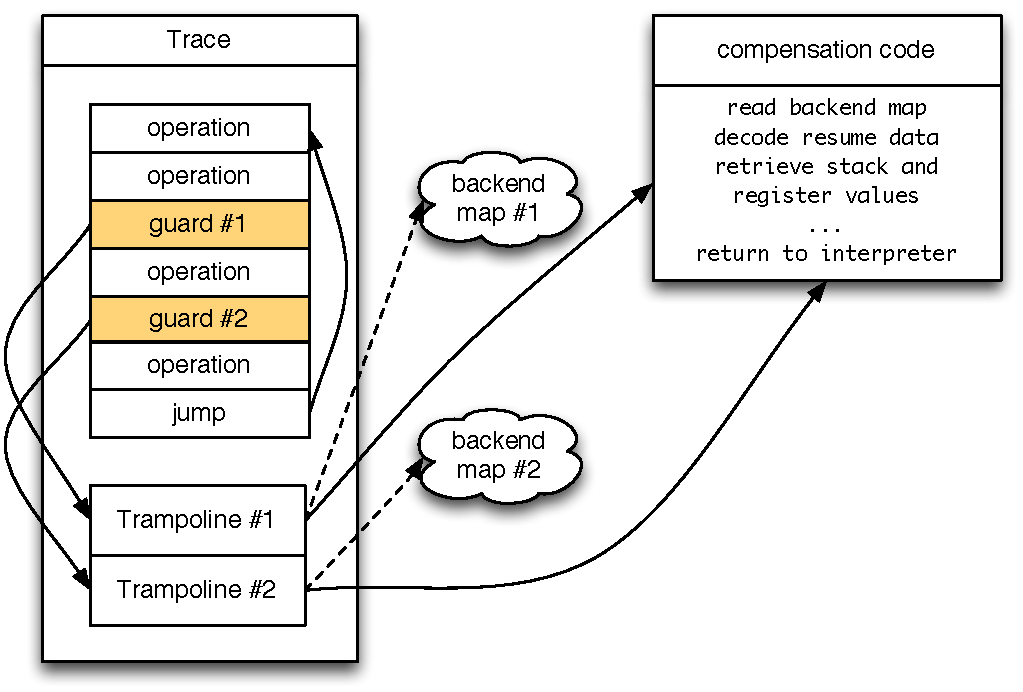
\includegraphics[width=1\textwidth]{figures/loop.pdf}
  \end{figure}
\end{frame}


\begin{frame}
  \frametitle{Compiling a Bridge}
  \begin{figure}
  \centering
  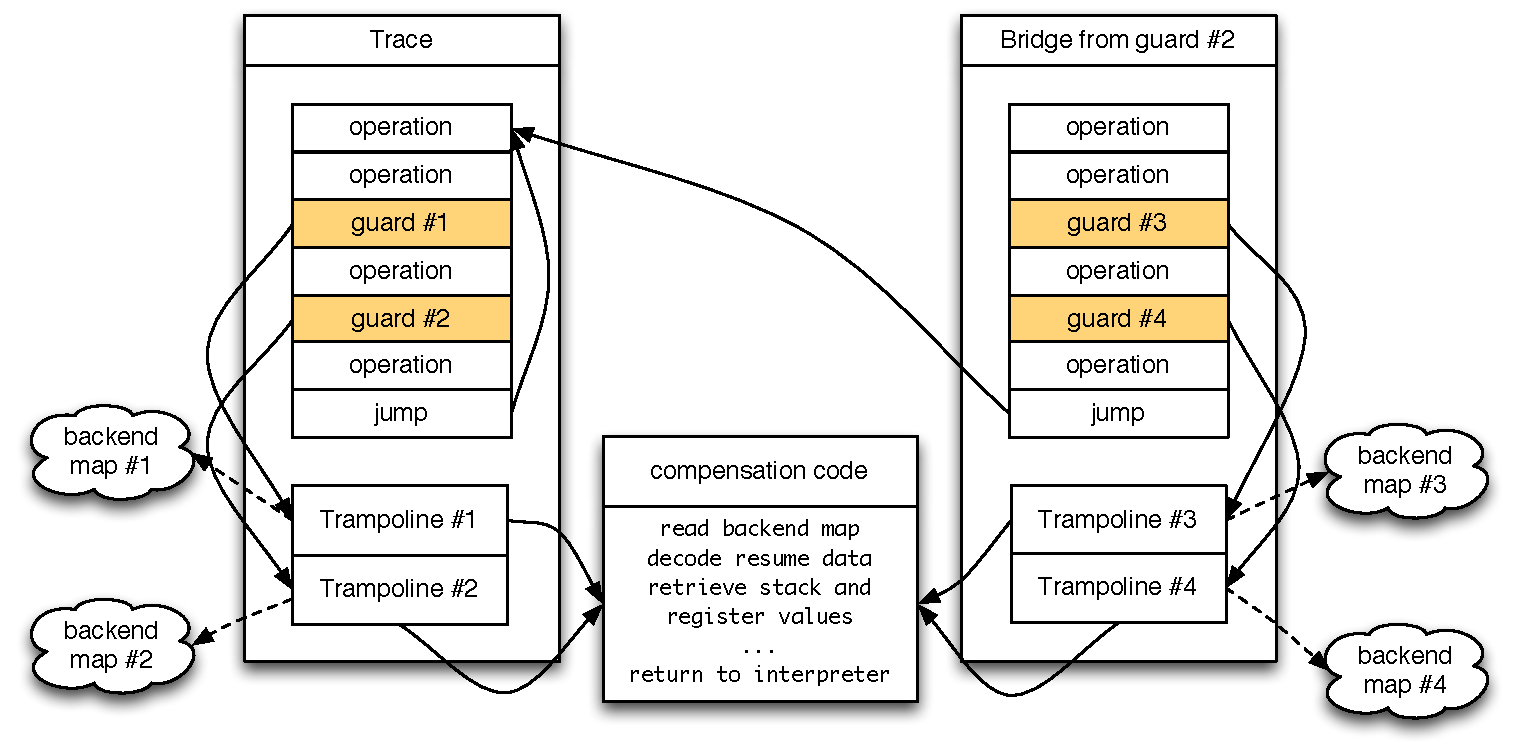
\includegraphics[width=1\textwidth]{figures/bridge_compiled.pdf}
  \end{figure}
\end{frame}
\begin{frame}
  \frametitle{Patching Guards for Bridges}
  \begin{figure}
  \centering
  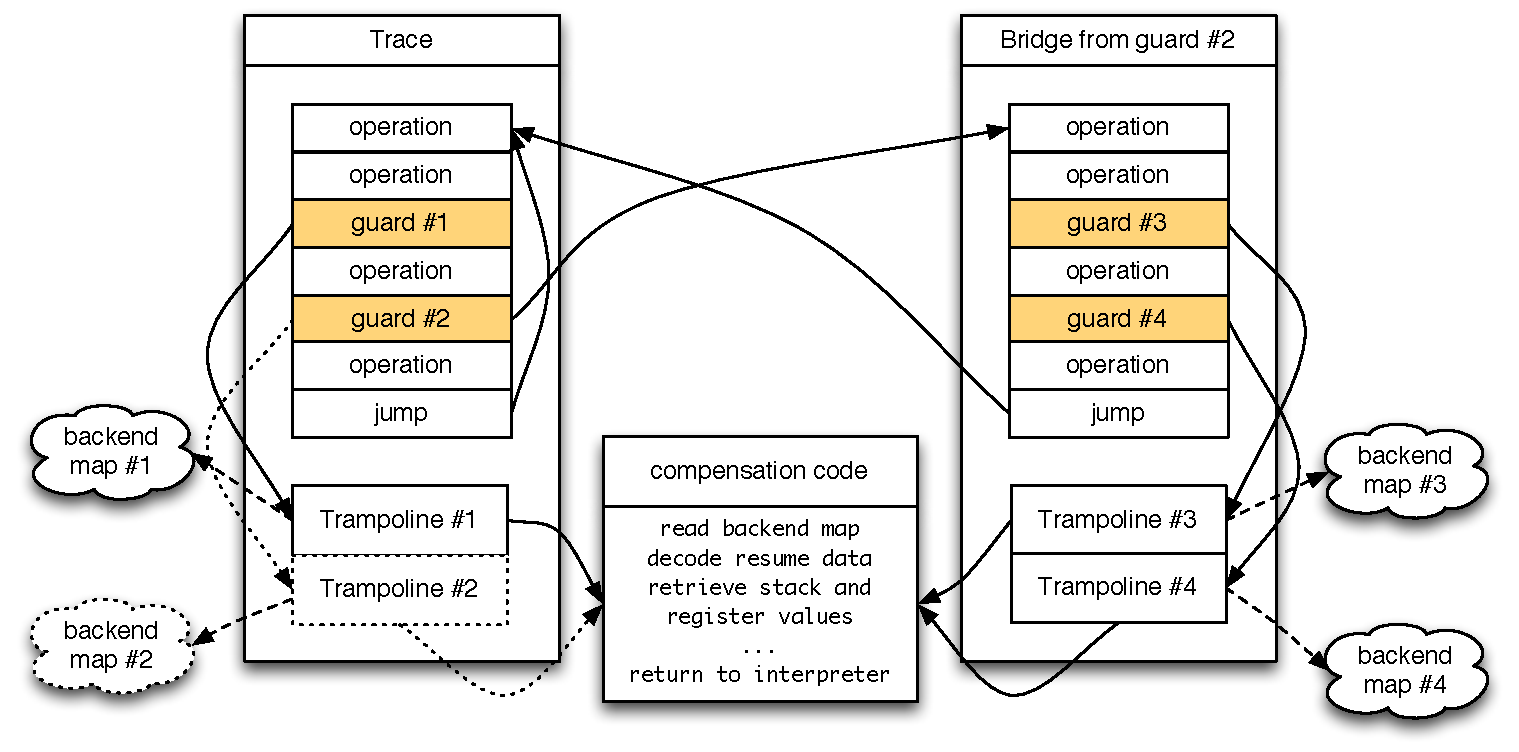
\includegraphics[width=1\textwidth]{figures/bridge_patched.pdf}
  \end{figure}
\end{frame}
\begin{frame}[t,fragile]
\pgfplotsset{tick label style={font=\tiny\bfseries},
label style={font=\small},
legend style={font=\tiny}
}
    \frametitle{Guard Failure Rates}
    \begin{figure}
        \centering
        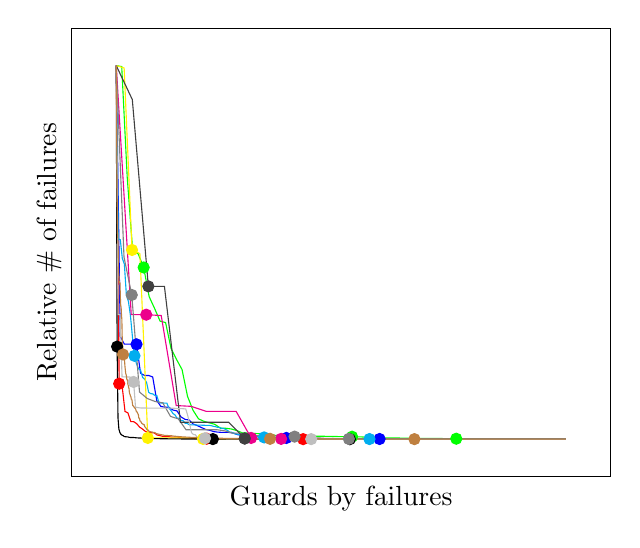
\begin{tikzpicture}
            \begin{axis}[
            xlabel= Guards by failures,
            ylabel=Relative \# of failures,
            xtick=\empty,
            ytick=\empty,
            ]
                
\addplot[red,mark=none] coordinates {
(0.000000,1.000000) (0.006494,0.148545) (0.012987,0.143156) (0.019481,0.074262) (0.025974,0.070332) (0.032468,0.047160) (0.038961,0.046744) (0.045455,0.041526) (0.051948,0.032187) (0.058442,0.027040) (0.064935,0.020597) (0.071429,0.018534) (0.077922,0.017118) (0.084416,0.016888) (0.090909,0.011212) (0.097403,0.009493) (0.103896,0.007359) (0.110390,0.007268) (0.116883,0.006596) (0.123377,0.005563) (0.129870,0.005529) (0.136364,0.005470) (0.142857,0.003591) (0.149351,0.002948) (0.155844,0.002945) (0.162338,0.002749) (0.168831,0.002558) (0.175325,0.001651) (0.181818,0.001644) (0.188312,0.001592) (0.194805,0.001582) (0.201299,0.001365) (0.207792,0.001362) (0.214286,0.000933) (0.220779,0.000887) (0.227273,0.000871) (0.233766,0.000863) (0.240260,0.000843) (0.246753,0.000726) (0.253247,0.000695) (0.259740,0.000594) (0.266234,0.000558) (0.272727,0.000534) (0.279221,0.000498) (0.285714,0.000389) (0.292208,0.000389) (0.298701,0.000382) (0.305195,0.000381) (0.311688,0.000376) (0.318182,0.000364) (0.324675,0.000340) (0.331169,0.000312) (0.337662,0.000237) (0.344156,0.000219) (0.350649,0.000204) (0.357143,0.000202) (0.363636,0.000202) (0.370130,0.000193) (0.376623,0.000174) (0.383117,0.000162) (0.389610,0.000139) (0.396104,0.000137) (0.402597,0.000135) (0.409091,0.000130) (0.415584,0.000130) (0.422078,0.000122) (0.428571,0.000119) (0.435065,0.000104) (0.441558,0.000101) (0.448052,0.000097) (0.454545,0.000087) (0.461039,0.000079) (0.467532,0.000069) (0.474026,0.000058) (0.480519,0.000051) (0.487013,0.000041) (0.493506,0.000040) (0.500000,0.000035) (0.506494,0.000029) (0.512987,0.000028) (0.519481,0.000028) (0.525974,0.000027) (0.532468,0.000026) (0.538961,0.000026) (0.545455,0.000024) (0.551948,0.000021) (0.558442,0.000018) (0.564935,0.000018) (0.571429,0.000017) (0.577922,0.000016) (0.584416,0.000015) (0.590909,0.000015) (0.597403,0.000014) (0.603896,0.000014) (0.610390,0.000011) (0.616883,0.000011) (0.623377,0.000011) (0.629870,0.000011) (0.636364,0.000011) (0.642857,0.000011) (0.649351,0.000011) (0.655844,0.000011) (0.662338,0.000010) (0.668831,0.000009) (0.675325,0.000007) (0.681818,0.000007) (0.688312,0.000007) (0.694805,0.000007) (0.701299,0.000007) (0.707792,0.000006) (0.714286,0.000006) (0.720779,0.000005) (0.727273,0.000005) (0.733766,0.000005) (0.740260,0.000005) (0.746753,0.000004) (0.753247,0.000004) (0.759740,0.000003) (0.766234,0.000003) (0.772727,0.000003) (0.779221,0.000003) (0.785714,0.000002) (0.792208,0.000002) (0.798701,0.000002) (0.805195,0.000002) (0.811688,0.000002) (0.818182,0.000002) (0.824675,0.000002) (0.831169,0.000002) (0.837662,0.000002) (0.844156,0.000002) (0.850649,0.000002) (0.857143,0.000002) (0.863636,0.000002) (0.870130,0.000001) (0.876623,0.000001) (0.883117,0.000001) (0.889610,0.000001) (0.896104,0.000001) (0.902597,0.000001) (0.909091,0.000001) (0.915584,0.000001) (0.922078,0.000001) (0.928571,0.000001) (0.935065,0.000001) (0.941558,0.000001) (0.948052,0.000000) (0.954545,0.000000) (0.961039,0.000000) (0.967532,0.000000) (0.974026,0.000000) (0.980519,0.000000) (0.987013,0.000000) (0.993506,0.000000) (1.000000,0.000000)
};
\addplot[red,only marks,mark=*] coordinates {(0.006494,0.148545) (0.201299,0.001365) (0.415584,0.000130)};
    
\addplot[green,mark=none] coordinates {
(0.000000,1.000000) (0.012195,0.997326) (0.024390,0.701335) (0.036585,0.503352) (0.048780,0.496172) (0.060976,0.459611) (0.073171,0.381570) (0.085366,0.349645) (0.097561,0.315892) (0.109756,0.312117) (0.121951,0.242322) (0.134146,0.213275) (0.146341,0.186336) (0.158537,0.114441) (0.170732,0.077514) (0.182927,0.054374) (0.195122,0.047764) (0.207317,0.043576) (0.219512,0.039644) (0.231707,0.029204) (0.243902,0.029145) (0.256098,0.027214) (0.268293,0.023030) (0.280488,0.016877) (0.292683,0.016283) (0.304878,0.015489) (0.317073,0.014624) (0.329268,0.014572) (0.341463,0.014451) (0.353659,0.009960) (0.365854,0.009811) (0.378049,0.009299) (0.390244,0.009197) (0.402439,0.009182) (0.414634,0.009178) (0.426829,0.007813) (0.439024,0.007797) (0.451220,0.007786) (0.463415,0.007715) (0.475610,0.007381) (0.487805,0.007172) (0.500000,0.006791) (0.512195,0.006783) (0.524390,0.006634) (0.536585,0.006366) (0.548780,0.005879) (0.560976,0.004203) (0.573171,0.004074) (0.585366,0.003983) (0.597561,0.003260) (0.609756,0.003252) (0.621951,0.003181) (0.634146,0.002945) (0.646341,0.002670) (0.658537,0.002399) (0.670732,0.002159) (0.682927,0.002143) (0.695122,0.001817) (0.707317,0.001793) (0.719512,0.001785) (0.731707,0.001577) (0.743902,0.001573) (0.756098,0.001243) (0.768293,0.001073) (0.780488,0.000598) (0.792683,0.000590) (0.804878,0.000492) (0.817073,0.000440) (0.829268,0.000240) (0.841463,0.000201) (0.853659,0.000201) (0.865854,0.000197) (0.878049,0.000177) (0.890244,0.000079) (0.902439,0.000079) (0.914634,0.000067) (0.926829,0.000031) (0.939024,0.000028) (0.951220,0.000024) (0.963415,0.000012) (0.975610,0.000008) (0.987805,0.000004) (1.000000,0.000004)
};
\addplot[green,only marks,mark=*] coordinates {(0.060976,0.459611) (0.524390,0.006634) (0.756098,0.001243)};
    
\addplot[blue,mark=none] coordinates {
(0.000000,1.000000) (0.009009,0.274799) (0.018018,0.254401) (0.027027,0.254401) (0.036036,0.254400) (0.045045,0.253942) (0.054054,0.176493) (0.063063,0.170575) (0.072072,0.170575) (0.081081,0.166477) (0.090090,0.103439) (0.099099,0.087880) (0.108108,0.085545) (0.117117,0.085441) (0.126126,0.077913) (0.135135,0.075639) (0.144144,0.059419) (0.153153,0.052926) (0.162162,0.051446) (0.171171,0.040551) (0.180180,0.036356) (0.189189,0.031443) (0.198198,0.026162) (0.207207,0.023960) (0.216216,0.020391) (0.225225,0.018926) (0.234234,0.018265) (0.243243,0.018091) (0.252252,0.018011) (0.261261,0.015999) (0.270270,0.011937) (0.279279,0.010101) (0.288288,0.010101) (0.297297,0.009964) (0.306306,0.009956) (0.315315,0.009498) (0.324324,0.006923) (0.333333,0.006919) (0.342342,0.005088) (0.351351,0.004699) (0.360360,0.004400) (0.369369,0.004132) (0.378378,0.003324) (0.387387,0.003266) (0.396396,0.003017) (0.405405,0.002900) (0.414414,0.002389) (0.423423,0.001747) (0.432432,0.001717) (0.441441,0.001660) (0.450450,0.001634) (0.459459,0.001542) (0.468468,0.001353) (0.477477,0.001264) (0.486486,0.001263) (0.495495,0.001131) (0.504505,0.001046) (0.513514,0.000934) (0.522523,0.000928) (0.531532,0.000856) (0.540541,0.000850) (0.549550,0.000821) (0.558559,0.000745) (0.567568,0.000679) (0.576577,0.000581) (0.585586,0.000480) (0.594595,0.000316) (0.603604,0.000260) (0.612613,0.000256) (0.621622,0.000209) (0.630631,0.000195) (0.639640,0.000163) (0.648649,0.000161) (0.657658,0.000145) (0.666667,0.000136) (0.675676,0.000134) (0.684685,0.000128) (0.693694,0.000123) (0.702703,0.000117) (0.711712,0.000100) (0.720721,0.000099) (0.729730,0.000095) (0.738739,0.000088) (0.747748,0.000087) (0.756757,0.000065) (0.765766,0.000058) (0.774775,0.000052) (0.783784,0.000051) (0.792793,0.000045) (0.801802,0.000043) (0.810811,0.000033) (0.819820,0.000031) (0.828829,0.000028) (0.837838,0.000023) (0.846847,0.000019) (0.855856,0.000018) (0.864865,0.000017) (0.873874,0.000017) (0.882883,0.000016) (0.891892,0.000016) (0.900901,0.000016) (0.909910,0.000016) (0.918919,0.000015) (0.927928,0.000015) (0.936937,0.000012) (0.945946,0.000011) (0.954955,0.000009) (0.963964,0.000006) (0.972973,0.000005) (0.981982,0.000003) (0.990991,0.000001) (1.000000,0.000000)
};
\addplot[blue,only marks,mark=*] coordinates {(0.045045,0.253942) (0.378378,0.003324) (0.585586,0.000480)};
    
\addplot[cyan,mark=none] coordinates {
(0.000000,1.000000) (0.004505,0.536162) (0.009009,0.533859) (0.013514,0.483711) (0.018018,0.468958) (0.022523,0.385926) (0.027027,0.368855) (0.031532,0.330881) (0.036036,0.273385) (0.040541,0.223088) (0.045045,0.201529) (0.049550,0.188300) (0.054054,0.184877) (0.058559,0.165360) (0.063063,0.160965) (0.067568,0.151293) (0.072072,0.125402) (0.076577,0.121903) (0.081081,0.121395) (0.085586,0.117212) (0.090090,0.117117) (0.094595,0.099425) (0.099099,0.096936) (0.103604,0.096847) (0.108108,0.096552) (0.112613,0.096421) (0.117117,0.083108) (0.121622,0.076876) (0.126126,0.068604) (0.130631,0.064969) (0.135135,0.056385) (0.139640,0.056383) (0.144144,0.049812) (0.148649,0.049576) (0.153153,0.042719) (0.157658,0.042151) (0.162162,0.038817) (0.166667,0.038467) (0.171171,0.038437) (0.175676,0.038161) (0.180180,0.037712) (0.184685,0.037469) (0.189189,0.037434) (0.193694,0.037419) (0.198198,0.037035) (0.202703,0.037000) (0.207207,0.036987) (0.211712,0.035969) (0.216216,0.034370) (0.220721,0.033375) (0.225225,0.031819) (0.229730,0.031613) (0.234234,0.029056) (0.238739,0.028685) (0.243243,0.026102) (0.247748,0.023276) (0.252252,0.018629) (0.256757,0.018545) (0.261261,0.015560) (0.265766,0.013442) (0.270270,0.013322) (0.274775,0.011983) (0.279279,0.011599) (0.283784,0.008508) (0.288288,0.008463) (0.292793,0.008461) (0.297297,0.008456) (0.301802,0.007547) (0.306306,0.007021) (0.310811,0.006568) (0.315315,0.006344) (0.319820,0.005826) (0.324324,0.004751) (0.328829,0.004749) (0.333333,0.004749) (0.337838,0.003794) (0.342342,0.003082) (0.346847,0.002806) (0.351351,0.002767) (0.355856,0.002535) (0.360360,0.002472) (0.364865,0.002390) (0.369369,0.002320) (0.373874,0.002290) (0.378378,0.002275) (0.382883,0.002210) (0.387387,0.002049) (0.391892,0.001854) (0.396396,0.001647) (0.400901,0.001502) (0.405405,0.001322) (0.409910,0.001200) (0.414414,0.001161) (0.418919,0.001159) (0.423423,0.001146) (0.427928,0.001144) (0.432432,0.001116) (0.436937,0.001066) (0.441441,0.001059) (0.445946,0.001018) (0.450450,0.000873) (0.454955,0.000864) (0.459459,0.000840) (0.463964,0.000777) (0.468468,0.000766) (0.472973,0.000747) (0.477477,0.000729) (0.481982,0.000729) (0.486486,0.000621) (0.490991,0.000597) (0.495495,0.000590) (0.500000,0.000582) (0.504505,0.000577) (0.509009,0.000562) (0.513514,0.000558) (0.518018,0.000523) (0.522523,0.000478) (0.527027,0.000469) (0.531532,0.000456) (0.536036,0.000434) (0.540541,0.000432) (0.545045,0.000425) (0.549550,0.000425) (0.554054,0.000417) (0.558559,0.000412) (0.563063,0.000352) (0.567568,0.000332) (0.572072,0.000330) (0.576577,0.000326) (0.581081,0.000313) (0.585586,0.000289) (0.590090,0.000267) (0.594595,0.000247) (0.599099,0.000247) (0.603604,0.000217) (0.608108,0.000204) (0.612613,0.000195) (0.617117,0.000182) (0.621622,0.000165) (0.626126,0.000165) (0.630631,0.000163) (0.635135,0.000137) (0.639640,0.000137) (0.644144,0.000132) (0.648649,0.000130) (0.653153,0.000130) (0.657658,0.000122) (0.662162,0.000122) (0.666667,0.000122) (0.671171,0.000119) (0.675676,0.000115) (0.680180,0.000104) (0.684685,0.000104) (0.689189,0.000100) (0.693694,0.000096) (0.698198,0.000093) (0.702703,0.000087) (0.707207,0.000087) (0.711712,0.000087) (0.716216,0.000085) (0.720721,0.000085) (0.725225,0.000078) (0.729730,0.000074) (0.734234,0.000063) (0.738739,0.000059) (0.743243,0.000059) (0.747748,0.000059) (0.752252,0.000056) (0.756757,0.000056) (0.761261,0.000056) (0.765766,0.000054) (0.770270,0.000052) (0.774775,0.000052) (0.779279,0.000048) (0.783784,0.000046) (0.788288,0.000043) (0.792793,0.000041) (0.797297,0.000039) (0.801802,0.000039) (0.806306,0.000037) (0.810811,0.000037) (0.815315,0.000035) (0.819820,0.000035) (0.824324,0.000035) (0.828829,0.000033) (0.833333,0.000030) (0.837838,0.000030) (0.842342,0.000028) (0.846847,0.000028) (0.851351,0.000026) (0.855856,0.000026) (0.860360,0.000026) (0.864865,0.000024) (0.869369,0.000022) (0.873874,0.000020) (0.878378,0.000020) (0.882883,0.000017) (0.887387,0.000017) (0.891892,0.000017) (0.896396,0.000013) (0.900901,0.000013) (0.905405,0.000013) (0.909910,0.000011) (0.914414,0.000011) (0.918919,0.000011) (0.923423,0.000011) (0.927928,0.000011) (0.932432,0.000009) (0.936937,0.000009) (0.941441,0.000009) (0.945946,0.000009) (0.950450,0.000007) (0.954955,0.000007) (0.959459,0.000007) (0.963964,0.000004) (0.968468,0.000004) (0.972973,0.000004) (0.977477,0.000002) (0.981982,0.000002) (0.986486,0.000002) (0.990991,0.000002) (0.995495,0.000002) (1.000000,0.000002)
};
\addplot[cyan,only marks,mark=*] coordinates {(0.040541,0.223088) (0.328829,0.004749) (0.563063,0.000352)};
    
\addplot[magenta,mark=none] coordinates {
(0.000000,1.000000) (0.033333,0.333289) (0.066667,0.333230) (0.100000,0.330941) (0.133333,0.089999) (0.166667,0.087891) (0.200000,0.074485) (0.233333,0.074414) (0.266667,0.074281) (0.300000,0.003317) (0.333333,0.002204) (0.366667,0.000795) (0.400000,0.000294) (0.433333,0.000133) (0.466667,0.000099) (0.500000,0.000099) (0.533333,0.000067) (0.566667,0.000033) (0.600000,0.000032) (0.633333,0.000031) (0.666667,0.000025) (0.700000,0.000019) (0.733333,0.000010) (0.766667,0.000005) (0.800000,0.000003) (0.833333,0.000003) (0.866667,0.000003) (0.900000,0.000001) (0.933333,0.000001) (0.966667,0.000001) (1.000000,0.000001)
};
\addplot[magenta,only marks,mark=*] coordinates {(0.066667,0.333230) (0.300000,0.003317) (0.366667,0.000795)};
    
\addplot[yellow,mark=none] coordinates {
(0.000000,1.000000) (0.017544,0.993592) (0.035088,0.506431) (0.052632,0.496860) (0.070175,0.003334) (0.087719,0.003334) (0.105263,0.003290) (0.122807,0.003290) (0.140351,0.003290) (0.157895,0.003289) (0.175439,0.003250) (0.192982,0.000768) (0.210526,0.000464) (0.228070,0.000216) (0.245614,0.000205) (0.263158,0.000137) (0.280702,0.000133) (0.298246,0.000121) (0.315789,0.000105) (0.333333,0.000081) (0.350877,0.000067) (0.368421,0.000058) (0.385965,0.000055) (0.403509,0.000053) (0.421053,0.000052) (0.438596,0.000043) (0.456140,0.000034) (0.473684,0.000030) (0.491228,0.000029) (0.508772,0.000023) (0.526316,0.000022) (0.543860,0.000022) (0.561404,0.000022) (0.578947,0.000020) (0.596491,0.000019) (0.614035,0.000018) (0.631579,0.000014) (0.649123,0.000012) (0.666667,0.000011) (0.684211,0.000010) (0.701754,0.000006) (0.719298,0.000006) (0.736842,0.000005) (0.754386,0.000004) (0.771930,0.000004) (0.789474,0.000004) (0.807018,0.000003) (0.824561,0.000003) (0.842105,0.000002) (0.859649,0.000002) (0.877193,0.000001) (0.894737,0.000001) (0.912281,0.000001) (0.929825,0.000001) (0.947368,0.000000) (0.964912,0.000000) (0.982456,0.000000) (1.000000,0.000000)
};
\addplot[yellow,only marks,mark=*] coordinates {(0.035088,0.506431) (0.070175,0.003334) (0.192982,0.000768)};
    
\addplot[black,mark=none] coordinates {
(0.000000,1.000000) (0.001953,0.247783) (0.003906,0.056979) (0.005859,0.026968) (0.007812,0.019062) (0.009766,0.014136) (0.011719,0.011763) (0.013672,0.009968) (0.015625,0.009263) (0.017578,0.007132) (0.019531,0.006664) (0.021484,0.006547) (0.023438,0.006214) (0.025391,0.006190) (0.027344,0.005569) (0.029297,0.004773) (0.031250,0.004590) (0.033203,0.004576) (0.035156,0.004534) (0.037109,0.004497) (0.039062,0.004348) (0.041016,0.004135) (0.042969,0.003889) (0.044922,0.003631) (0.046875,0.003618) (0.048828,0.003285) (0.050781,0.003143) (0.052734,0.003024) (0.054688,0.003020) (0.056641,0.002903) (0.058594,0.002661) (0.060547,0.002589) (0.062500,0.002268) (0.064453,0.002194) (0.066406,0.002187) (0.068359,0.001941) (0.070312,0.001798) (0.072266,0.001740) (0.074219,0.001716) (0.076172,0.001704) (0.078125,0.001658) (0.080078,0.001649) (0.082031,0.001550) (0.083984,0.001484) (0.085938,0.001468) (0.087891,0.001432) (0.089844,0.001429) (0.091797,0.001423) (0.093750,0.001376) (0.095703,0.001359) (0.097656,0.001281) (0.099609,0.001224) (0.101562,0.001212) (0.103516,0.001182) (0.105469,0.001181) (0.107422,0.001174) (0.109375,0.001089) (0.111328,0.001037) (0.113281,0.001024) (0.115234,0.000993) (0.117188,0.000955) (0.119141,0.000955) (0.121094,0.000954) (0.123047,0.000954) (0.125000,0.000902) (0.126953,0.000889) (0.128906,0.000887) (0.130859,0.000881) (0.132812,0.000856) (0.134766,0.000823) (0.136719,0.000694) (0.138672,0.000676) (0.140625,0.000675) (0.142578,0.000675) (0.144531,0.000625) (0.146484,0.000616) (0.148438,0.000603) (0.150391,0.000591) (0.152344,0.000575) (0.154297,0.000573) (0.156250,0.000553) (0.158203,0.000514) (0.160156,0.000491) (0.162109,0.000467) (0.164062,0.000429) (0.166016,0.000426) (0.167969,0.000426) (0.169922,0.000421) (0.171875,0.000419) (0.173828,0.000418) (0.175781,0.000413) (0.177734,0.000408) (0.179688,0.000408) (0.181641,0.000388) (0.183594,0.000385) (0.185547,0.000355) (0.187500,0.000336) (0.189453,0.000334) (0.191406,0.000324) (0.193359,0.000303) (0.195312,0.000296) (0.197266,0.000291) (0.199219,0.000267) (0.201172,0.000265) (0.203125,0.000264) (0.205078,0.000261) (0.207031,0.000260) (0.208984,0.000259) (0.210938,0.000259) (0.212891,0.000251) (0.214844,0.000248) (0.216797,0.000245) (0.218750,0.000237) (0.220703,0.000215) (0.222656,0.000209) (0.224609,0.000208) (0.226562,0.000204) (0.228516,0.000201) (0.230469,0.000199) (0.232422,0.000197) (0.234375,0.000195) (0.236328,0.000179) (0.238281,0.000178) (0.240234,0.000178) (0.242188,0.000178) (0.244141,0.000178) (0.246094,0.000178) (0.248047,0.000178) (0.250000,0.000178) (0.251953,0.000171) (0.253906,0.000171) (0.255859,0.000170) (0.257812,0.000169) (0.259766,0.000166) (0.261719,0.000164) (0.263672,0.000163) (0.265625,0.000161) (0.267578,0.000160) (0.269531,0.000158) (0.271484,0.000155) (0.273438,0.000152) (0.275391,0.000148) (0.277344,0.000148) (0.279297,0.000148) (0.281250,0.000147) (0.283203,0.000147) (0.285156,0.000147) (0.287109,0.000146) (0.289062,0.000146) (0.291016,0.000145) (0.292969,0.000138) (0.294922,0.000136) (0.296875,0.000135) (0.298828,0.000134) (0.300781,0.000133) (0.302734,0.000132) (0.304688,0.000127) (0.306641,0.000125) (0.308594,0.000125) (0.310547,0.000124) (0.312500,0.000122) (0.314453,0.000121) (0.316406,0.000120) (0.318359,0.000119) (0.320312,0.000118) (0.322266,0.000118) (0.324219,0.000113) (0.326172,0.000110) (0.328125,0.000109) (0.330078,0.000107) (0.332031,0.000106) (0.333984,0.000104) (0.335938,0.000102) (0.337891,0.000097) (0.339844,0.000095) (0.341797,0.000092) (0.343750,0.000091) (0.345703,0.000089) (0.347656,0.000088) (0.349609,0.000086) (0.351562,0.000086) (0.353516,0.000086) (0.355469,0.000085) (0.357422,0.000085) (0.359375,0.000084) (0.361328,0.000083) (0.363281,0.000081) (0.365234,0.000081) (0.367188,0.000081) (0.369141,0.000077) (0.371094,0.000076) (0.373047,0.000076) (0.375000,0.000075) (0.376953,0.000074) (0.378906,0.000074) (0.380859,0.000067) (0.382812,0.000066) (0.384766,0.000065) (0.386719,0.000065) (0.388672,0.000062) (0.390625,0.000060) (0.392578,0.000055) (0.394531,0.000055) (0.396484,0.000051) (0.398438,0.000049) (0.400391,0.000049) (0.402344,0.000048) (0.404297,0.000046) (0.406250,0.000045) (0.408203,0.000044) (0.410156,0.000044) (0.412109,0.000044) (0.414062,0.000043) (0.416016,0.000042) (0.417969,0.000042) (0.419922,0.000041) (0.421875,0.000040) (0.423828,0.000040) (0.425781,0.000040) (0.427734,0.000038) (0.429688,0.000038) (0.431641,0.000037) (0.433594,0.000036) (0.435547,0.000035) (0.437500,0.000035) (0.439453,0.000034) (0.441406,0.000034) (0.443359,0.000034) (0.445312,0.000033) (0.447266,0.000032) (0.449219,0.000031) (0.451172,0.000031) (0.453125,0.000031) (0.455078,0.000029) (0.457031,0.000028) (0.458984,0.000027) (0.460938,0.000027) (0.462891,0.000027) (0.464844,0.000027) (0.466797,0.000026) (0.468750,0.000025) (0.470703,0.000025) (0.472656,0.000025) (0.474609,0.000024) (0.476562,0.000024) (0.478516,0.000023) (0.480469,0.000023) (0.482422,0.000023) (0.484375,0.000023) (0.486328,0.000023) (0.488281,0.000023) (0.490234,0.000023) (0.492188,0.000023) (0.494141,0.000023) (0.496094,0.000023) (0.498047,0.000023) (0.500000,0.000023) (0.501953,0.000023) (0.503906,0.000022) (0.505859,0.000022) (0.507812,0.000022) (0.509766,0.000022) (0.511719,0.000022) (0.513672,0.000021) (0.515625,0.000021) (0.517578,0.000021) (0.519531,0.000021) (0.521484,0.000021) (0.523438,0.000021) (0.525391,0.000021) (0.527344,0.000020) (0.529297,0.000020) (0.531250,0.000019) (0.533203,0.000019) (0.535156,0.000019) (0.537109,0.000019) (0.539062,0.000018) (0.541016,0.000018) (0.542969,0.000018) (0.544922,0.000018) (0.546875,0.000018) (0.548828,0.000018) (0.550781,0.000017) (0.552734,0.000017) (0.554688,0.000017) (0.556641,0.000017) (0.558594,0.000017) (0.560547,0.000016) (0.562500,0.000016) (0.564453,0.000016) (0.566406,0.000015) (0.568359,0.000015) (0.570312,0.000015) (0.572266,0.000015) (0.574219,0.000014) (0.576172,0.000014) (0.578125,0.000014) (0.580078,0.000014) (0.582031,0.000013) (0.583984,0.000013) (0.585938,0.000013) (0.587891,0.000013) (0.589844,0.000013) (0.591797,0.000012) (0.593750,0.000012) (0.595703,0.000012) (0.597656,0.000012) (0.599609,0.000012) (0.601562,0.000012) (0.603516,0.000012) (0.605469,0.000012) (0.607422,0.000011) (0.609375,0.000011) (0.611328,0.000011) (0.613281,0.000011) (0.615234,0.000011) (0.617188,0.000011) (0.619141,0.000011) (0.621094,0.000010) (0.623047,0.000010) (0.625000,0.000009) (0.626953,0.000009) (0.628906,0.000009) (0.630859,0.000009) (0.632812,0.000009) (0.634766,0.000009) (0.636719,0.000009) (0.638672,0.000009) (0.640625,0.000009) (0.642578,0.000009) (0.644531,0.000009) (0.646484,0.000009) (0.648438,0.000009) (0.650391,0.000009) (0.652344,0.000009) (0.654297,0.000009) (0.656250,0.000009) (0.658203,0.000009) (0.660156,0.000009) (0.662109,0.000009) (0.664062,0.000009) (0.666016,0.000009) (0.667969,0.000009) (0.669922,0.000008) (0.671875,0.000008) (0.673828,0.000008) (0.675781,0.000008) (0.677734,0.000008) (0.679688,0.000008) (0.681641,0.000008) (0.683594,0.000008) (0.685547,0.000008) (0.687500,0.000008) (0.689453,0.000008) (0.691406,0.000008) (0.693359,0.000008) (0.695312,0.000008) (0.697266,0.000008) (0.699219,0.000007) (0.701172,0.000007) (0.703125,0.000007) (0.705078,0.000007) (0.707031,0.000007) (0.708984,0.000007) (0.710938,0.000007) (0.712891,0.000007) (0.714844,0.000006) (0.716797,0.000006) (0.718750,0.000006) (0.720703,0.000006) (0.722656,0.000006) (0.724609,0.000006) (0.726562,0.000006) (0.728516,0.000006) (0.730469,0.000006) (0.732422,0.000005) (0.734375,0.000005) (0.736328,0.000005) (0.738281,0.000005) (0.740234,0.000005) (0.742188,0.000005) (0.744141,0.000005) (0.746094,0.000005) (0.748047,0.000005) (0.750000,0.000005) (0.751953,0.000005) (0.753906,0.000005) (0.755859,0.000004) (0.757812,0.000004) (0.759766,0.000004) (0.761719,0.000004) (0.763672,0.000004) (0.765625,0.000004) (0.767578,0.000004) (0.769531,0.000004) (0.771484,0.000004) (0.773438,0.000004) (0.775391,0.000004) (0.777344,0.000004) (0.779297,0.000004) (0.781250,0.000004) (0.783203,0.000004) (0.785156,0.000004) (0.787109,0.000004) (0.789062,0.000004) (0.791016,0.000004) (0.792969,0.000004) (0.794922,0.000004) (0.796875,0.000004) (0.798828,0.000004) (0.800781,0.000004) (0.802734,0.000003) (0.804688,0.000003) (0.806641,0.000003) (0.808594,0.000003) (0.810547,0.000003) (0.812500,0.000003) (0.814453,0.000003) (0.816406,0.000003) (0.818359,0.000003) (0.820312,0.000003) (0.822266,0.000003) (0.824219,0.000003) (0.826172,0.000003) (0.828125,0.000003) (0.830078,0.000003) (0.832031,0.000003) (0.833984,0.000003) (0.835938,0.000003) (0.837891,0.000003) (0.839844,0.000003) (0.841797,0.000003) (0.843750,0.000003) (0.845703,0.000003) (0.847656,0.000003) (0.849609,0.000003) (0.851562,0.000003) (0.853516,0.000002) (0.855469,0.000002) (0.857422,0.000002) (0.859375,0.000002) (0.861328,0.000002) (0.863281,0.000002) (0.865234,0.000002) (0.867188,0.000002) (0.869141,0.000002) (0.871094,0.000002) (0.873047,0.000002) (0.875000,0.000002) (0.876953,0.000002) (0.878906,0.000002) (0.880859,0.000002) (0.882812,0.000002) (0.884766,0.000002) (0.886719,0.000002) (0.888672,0.000002) (0.890625,0.000002) (0.892578,0.000002) (0.894531,0.000002) (0.896484,0.000002) (0.898438,0.000002) (0.900391,0.000001) (0.902344,0.000001) (0.904297,0.000001) (0.906250,0.000001) (0.908203,0.000001) (0.910156,0.000001) (0.912109,0.000001) (0.914062,0.000001) (0.916016,0.000001) (0.917969,0.000001) (0.919922,0.000001) (0.921875,0.000001) (0.923828,0.000001) (0.925781,0.000001) (0.927734,0.000001) (0.929688,0.000001) (0.931641,0.000001) (0.933594,0.000001) (0.935547,0.000001) (0.937500,0.000001) (0.939453,0.000001) (0.941406,0.000001) (0.943359,0.000001) (0.945312,0.000001) (0.947266,0.000001) (0.949219,0.000001) (0.951172,0.000001) (0.953125,0.000001) (0.955078,0.000001) (0.957031,0.000001) (0.958984,0.000001) (0.960938,0.000000) (0.962891,0.000000) (0.964844,0.000000) (0.966797,0.000000) (0.968750,0.000000) (0.970703,0.000000) (0.972656,0.000000) (0.974609,0.000000) (0.976562,0.000000) (0.978516,0.000000) (0.980469,0.000000) (0.982422,0.000000) (0.984375,0.000000) (0.986328,0.000000) (0.988281,0.000000) (0.990234,0.000000) (0.992188,0.000000) (0.994141,0.000000) (0.996094,0.000000) (0.998047,0.000000) (1.000000,0.000000)
};
\addplot[black,only marks,mark=*] coordinates {(0.001953,0.247783) (0.214844,0.000248) (0.519531,0.000021)};
    
\addplot[gray,mark=none] coordinates {
(0.000000,1.000000) (0.017241,0.487558) (0.034483,0.386091) (0.051724,0.126229) (0.068966,0.108863) (0.086207,0.100941) (0.103448,0.097250) (0.120690,0.060934) (0.137931,0.054349) (0.155172,0.025283) (0.172414,0.025270) (0.189655,0.025262) (0.206897,0.025238) (0.224138,0.025208) (0.241379,0.022267) (0.258621,0.016262) (0.275862,0.016261) (0.293103,0.012610) (0.310345,0.009401) (0.327586,0.008822) (0.344828,0.008804) (0.362069,0.008801) (0.379310,0.007326) (0.396552,0.006830) (0.413793,0.003673) (0.431034,0.003672) (0.448276,0.003642) (0.465517,0.001939) (0.482759,0.001709) (0.500000,0.000965) (0.517241,0.000962) (0.534483,0.000277) (0.551724,0.000119) (0.568966,0.000093) (0.586207,0.000088) (0.603448,0.000050) (0.620690,0.000048) (0.637931,0.000043) (0.655172,0.000042) (0.672414,0.000025) (0.689655,0.000021) (0.706897,0.000011) (0.724138,0.000011) (0.741379,0.000011) (0.758621,0.000011) (0.775862,0.000011) (0.793103,0.000010) (0.810345,0.000009) (0.827586,0.000008) (0.844828,0.000006) (0.862069,0.000005) (0.879310,0.000004) (0.896552,0.000003) (0.913793,0.000002) (0.931034,0.000002) (0.948276,0.000001) (0.965517,0.000001) (0.982759,0.000001) (1.000000,0.000000)
};
\addplot[gray,only marks,mark=*] coordinates {(0.034483,0.386091) (0.396552,0.006830) (0.517241,0.000962)};
    
\addplot[darkgray,mark=none] coordinates {
(0.000000,1.000000) (0.035714,0.909090) (0.071429,0.409043) (0.107143,0.409043) (0.142857,0.045445) (0.178571,0.045445) (0.214286,0.045437) (0.250000,0.045437) (0.285714,0.001856) (0.321429,0.000157) (0.357143,0.000150) (0.392857,0.000148) (0.428571,0.000138) (0.464286,0.000116) (0.500000,0.000070) (0.535714,0.000048) (0.571429,0.000032) (0.607143,0.000032) (0.642857,0.000032) (0.678571,0.000016) (0.714286,0.000009) (0.750000,0.000008) (0.785714,0.000008) (0.821429,0.000008) (0.857143,0.000006) (0.892857,0.000005) (0.928571,0.000002) (0.964286,0.000001) (1.000000,0.000001)
};
\addplot[darkgray,only marks,mark=*] coordinates {(0.071429,0.409043) (0.285714,0.001856) (0.285714,0.001856)};
    
\addplot[lightgray,mark=none] coordinates {
(0.000000,1.000000) (0.004292,0.333547) (0.008584,0.333312) (0.012876,0.166857) (0.017167,0.166758) (0.021459,0.166551) (0.025751,0.166414) (0.030043,0.166294) (0.034335,0.165678) (0.038627,0.153140) (0.042918,0.084910) (0.047210,0.084877) (0.051502,0.083928) (0.055794,0.083394) (0.060086,0.083329) (0.064378,0.083328) (0.068670,0.083313) (0.072961,0.083313) (0.077253,0.083302) (0.081545,0.083301) (0.085837,0.083292) (0.090129,0.083239) (0.094421,0.083209) (0.098712,0.083176) (0.103004,0.083169) (0.107296,0.083125) (0.111588,0.083071) (0.115880,0.083067) (0.120172,0.083054) (0.124464,0.082872) (0.128755,0.082758) (0.133047,0.082151) (0.137339,0.081810) (0.141631,0.081809) (0.145923,0.081721) (0.150215,0.081378) (0.154506,0.081001) (0.158798,0.063929) (0.163090,0.041639) (0.167382,0.017348) (0.171674,0.012510) (0.175966,0.011755) (0.180258,0.004971) (0.184549,0.004140) (0.188841,0.003972) (0.193133,0.002505) (0.197425,0.002447) (0.201717,0.002335) (0.206009,0.002075) (0.210300,0.001713) (0.214592,0.001685) (0.218884,0.001622) (0.223176,0.001588) (0.227468,0.001512) (0.231760,0.001506) (0.236052,0.001486) (0.240343,0.001475) (0.244635,0.001291) (0.248927,0.001284) (0.253219,0.001203) (0.257511,0.001158) (0.261803,0.001088) (0.266094,0.001087) (0.270386,0.001028) (0.274678,0.001019) (0.278970,0.001010) (0.283262,0.000943) (0.287554,0.000860) (0.291845,0.000808) (0.296137,0.000797) (0.300429,0.000788) (0.304721,0.000773) (0.309013,0.000769) (0.313305,0.000686) (0.317597,0.000640) (0.321888,0.000621) (0.326180,0.000604) (0.330472,0.000548) (0.334764,0.000478) (0.339056,0.000468) (0.343348,0.000444) (0.347639,0.000424) (0.351931,0.000419) (0.356223,0.000404) (0.360515,0.000388) (0.364807,0.000384) (0.369099,0.000381) (0.373391,0.000333) (0.377682,0.000327) (0.381974,0.000318) (0.386266,0.000301) (0.390558,0.000271) (0.394850,0.000262) (0.399142,0.000255) (0.403433,0.000243) (0.407725,0.000238) (0.412017,0.000237) (0.416309,0.000235) (0.420601,0.000230) (0.424893,0.000209) (0.429185,0.000189) (0.433476,0.000174) (0.437768,0.000165) (0.442060,0.000164) (0.446352,0.000153) (0.450644,0.000151) (0.454936,0.000150) (0.459227,0.000140) (0.463519,0.000136) (0.467811,0.000136) (0.472103,0.000118) (0.476395,0.000117) (0.480687,0.000112) (0.484979,0.000111) (0.489270,0.000106) (0.493562,0.000106) (0.497854,0.000106) (0.502146,0.000106) (0.506438,0.000106) (0.510730,0.000102) (0.515021,0.000092) (0.519313,0.000087) (0.523605,0.000082) (0.527897,0.000079) (0.532189,0.000077) (0.536481,0.000076) (0.540773,0.000075) (0.545064,0.000074) (0.549356,0.000073) (0.553648,0.000068) (0.557940,0.000068) (0.562232,0.000066) (0.566524,0.000063) (0.570815,0.000063) (0.575107,0.000062) (0.579399,0.000061) (0.583691,0.000061) (0.587983,0.000060) (0.592275,0.000059) (0.596567,0.000053) (0.600858,0.000050) (0.605150,0.000047) (0.609442,0.000046) (0.613734,0.000042) (0.618026,0.000042) (0.622318,0.000041) (0.626609,0.000040) (0.630901,0.000035) (0.635193,0.000035) (0.639485,0.000033) (0.643777,0.000033) (0.648069,0.000032) (0.652361,0.000032) (0.656652,0.000031) (0.660944,0.000031) (0.665236,0.000031) (0.669528,0.000031) (0.673820,0.000030) (0.678112,0.000029) (0.682403,0.000028) (0.686695,0.000027) (0.690987,0.000026) (0.695279,0.000025) (0.699571,0.000023) (0.703863,0.000022) (0.708155,0.000022) (0.712446,0.000021) (0.716738,0.000019) (0.721030,0.000018) (0.725322,0.000017) (0.729614,0.000016) (0.733906,0.000013) (0.738197,0.000012) (0.742489,0.000011) (0.746781,0.000011) (0.751073,0.000011) (0.755365,0.000011) (0.759657,0.000011) (0.763948,0.000011) (0.768240,0.000011) (0.772532,0.000011) (0.776824,0.000011) (0.781116,0.000011) (0.785408,0.000010) (0.789700,0.000010) (0.793991,0.000009) (0.798283,0.000009) (0.802575,0.000009) (0.806867,0.000009) (0.811159,0.000008) (0.815451,0.000007) (0.819742,0.000005) (0.824034,0.000005) (0.828326,0.000005) (0.832618,0.000005) (0.836910,0.000005) (0.841202,0.000004) (0.845494,0.000004) (0.849785,0.000004) (0.854077,0.000004) (0.858369,0.000004) (0.862661,0.000004) (0.866953,0.000004) (0.871245,0.000003) (0.875536,0.000003) (0.879828,0.000003) (0.884120,0.000003) (0.888412,0.000003) (0.892704,0.000002) (0.896996,0.000002) (0.901288,0.000002) (0.905579,0.000002) (0.909871,0.000002) (0.914163,0.000002) (0.918455,0.000001) (0.922747,0.000001) (0.927039,0.000001) (0.931330,0.000001) (0.935622,0.000001) (0.939914,0.000001) (0.944206,0.000001) (0.948498,0.000001) (0.952790,0.000001) (0.957082,0.000001) (0.961373,0.000001) (0.965665,0.000001) (0.969957,0.000001) (0.974249,0.000001) (0.978541,0.000001) (0.982833,0.000001) (0.987124,0.000001) (0.991416,0.000001) (0.995708,0.000001) (1.000000,0.000001)
};
\addplot[lightgray,only marks,mark=*] coordinates {(0.038627,0.153140) (0.197425,0.002447) (0.433476,0.000174)};
    
\addplot[brown,mark=none] coordinates {
(0.000000,1.000000) (0.000834,0.872400) (0.001668,0.683224) (0.002502,0.608314) (0.003336,0.542330) (0.004170,0.519721) (0.005004,0.447508) (0.005838,0.440065) (0.006672,0.420670) (0.007506,0.418862) (0.008340,0.418009) (0.009174,0.379519) (0.010008,0.357223) (0.010842,0.353534) (0.011676,0.333568) (0.012510,0.319704) (0.013344,0.268160) (0.014178,0.251065) (0.015013,0.226789) (0.015847,0.220089) (0.016681,0.215066) (0.017515,0.213903) (0.018349,0.213091) (0.019183,0.197153) (0.020017,0.187389) (0.020851,0.177430) (0.021685,0.173396) (0.022519,0.170787) (0.023353,0.160834) (0.024187,0.160045) (0.025021,0.157071) (0.025855,0.146612) (0.026689,0.144178) (0.027523,0.137699) (0.028357,0.136683) (0.029191,0.124833) (0.030025,0.121453) (0.030859,0.119189) (0.031693,0.115002) (0.032527,0.114249) (0.033361,0.107546) (0.034195,0.107268) (0.035029,0.104187) (0.035863,0.096624) (0.036697,0.089912) (0.037531,0.089585) (0.038365,0.087446) (0.039199,0.087298) (0.040033,0.084823) (0.040867,0.083414) (0.041701,0.083212) (0.042535,0.082227) (0.043369,0.079913) (0.044204,0.075734) (0.045038,0.073337) (0.045872,0.073039) (0.046706,0.072381) (0.047540,0.069693) (0.048374,0.067325) (0.049208,0.065996) (0.050042,0.057532) (0.050876,0.055707) (0.051710,0.055669) (0.052544,0.049083) (0.053378,0.048652) (0.054212,0.048015) (0.055046,0.045918) (0.055880,0.045234) (0.056714,0.042272) (0.057548,0.041798) (0.058382,0.040969) (0.059216,0.040163) (0.060050,0.040016) (0.060884,0.038778) (0.061718,0.038686) (0.062552,0.038456) (0.063386,0.033439) (0.064220,0.032381) (0.065054,0.031115) (0.065888,0.030103) (0.066722,0.029385) (0.067556,0.026654) (0.068390,0.025877) (0.069224,0.024467) (0.070058,0.024427) (0.070892,0.024134) (0.071726,0.024036) (0.072560,0.021379) (0.073394,0.020813) (0.074229,0.020166) (0.075063,0.020056) (0.075897,0.019981) (0.076731,0.019791) (0.077565,0.019672) (0.078399,0.019356) (0.079233,0.019269) (0.080067,0.019134) (0.080901,0.018119) (0.081735,0.017905) (0.082569,0.017878) (0.083403,0.017865) (0.084237,0.017769) (0.085071,0.017758) (0.085905,0.017065) (0.086739,0.016959) (0.087573,0.016686) (0.088407,0.015666) (0.089241,0.014908) (0.090075,0.014542) (0.090909,0.014518) (0.091743,0.014200) (0.092577,0.013865) (0.093411,0.013736) (0.094245,0.013273) (0.095079,0.013197) (0.095913,0.012997) (0.096747,0.012759) (0.097581,0.012642) (0.098415,0.012344) (0.099249,0.012031) (0.100083,0.011973) (0.100917,0.011805) (0.101751,0.011594) (0.102585,0.011387) (0.103420,0.011332) (0.104254,0.011246) (0.105088,0.010925) (0.105922,0.010566) (0.106756,0.010269) (0.107590,0.010235) (0.108424,0.010220) (0.109258,0.010135) (0.110092,0.010071) (0.110926,0.010048) (0.111760,0.010002) (0.112594,0.009762) (0.113428,0.009756) (0.114262,0.009751) (0.115096,0.009730) (0.115930,0.009551) (0.116764,0.009536) (0.117598,0.009404) (0.118432,0.009399) (0.119266,0.009298) (0.120100,0.009263) (0.120934,0.009245) (0.121768,0.009137) (0.122602,0.009120) (0.123436,0.009097) (0.124270,0.008816) (0.125104,0.008646) (0.125938,0.008484) (0.126772,0.008405) (0.127606,0.008149) (0.128440,0.008032) (0.129274,0.007872) (0.130108,0.007866) (0.130942,0.007823) (0.131776,0.007801) (0.132611,0.007718) (0.133445,0.007481) (0.134279,0.007373) (0.135113,0.007345) (0.135947,0.007296) (0.136781,0.007269) (0.137615,0.007233) (0.138449,0.006991) (0.139283,0.006905) (0.140117,0.006795) (0.140951,0.006738) (0.141785,0.006708) (0.142619,0.006551) (0.143453,0.006510) (0.144287,0.006435) (0.145121,0.006361) (0.145955,0.006238) (0.146789,0.006134) (0.147623,0.006027) (0.148457,0.005991) (0.149291,0.005921) (0.150125,0.005852) (0.150959,0.005852) (0.151793,0.005823) (0.152627,0.005794) (0.153461,0.005787) (0.154295,0.005746) (0.155129,0.005672) (0.155963,0.005619) (0.156797,0.005612) (0.157631,0.005557) (0.158465,0.005495) (0.159299,0.005495) (0.160133,0.005422) (0.160967,0.005324) (0.161802,0.005217) (0.162636,0.005196) (0.163470,0.005167) (0.164304,0.005107) (0.165138,0.005012) (0.165972,0.004999) (0.166806,0.004985) (0.167640,0.004981) (0.168474,0.004936) (0.169308,0.004912) (0.170142,0.004836) (0.170976,0.004822) (0.171810,0.004755) (0.172644,0.004692) (0.173478,0.004687) (0.174312,0.004667) (0.175146,0.004605) (0.175980,0.004546) (0.176814,0.004523) (0.177648,0.004518) (0.178482,0.004512) (0.179316,0.004447) (0.180150,0.004427) (0.180984,0.004408) (0.181818,0.004401) (0.182652,0.004336) (0.183486,0.004326) (0.184320,0.004255) (0.185154,0.004163) (0.185988,0.004152) (0.186822,0.004150) (0.187656,0.004132) (0.188490,0.004125) (0.189324,0.003972) (0.190158,0.003971) (0.190992,0.003942) (0.191827,0.003842) (0.192661,0.003797) (0.193495,0.003710) (0.194329,0.003703) (0.195163,0.003684) (0.195997,0.003626) (0.196831,0.003620) (0.197665,0.003576) (0.198499,0.003526) (0.199333,0.003451) (0.200167,0.003447) (0.201001,0.003402) (0.201835,0.003390) (0.202669,0.003364) (0.203503,0.003361) (0.204337,0.003356) (0.205171,0.003350) (0.206005,0.003341) (0.206839,0.003321) (0.207673,0.003278) (0.208507,0.003246) (0.209341,0.003239) (0.210175,0.003219) (0.211009,0.003208) (0.211843,0.003129) (0.212677,0.003123) (0.213511,0.003073) (0.214345,0.003063) (0.215179,0.003053) (0.216013,0.003053) (0.216847,0.003026) (0.217681,0.003007) (0.218515,0.002989) (0.219349,0.002929) (0.220183,0.002915) (0.221018,0.002913) (0.221852,0.002890) (0.222686,0.002861) (0.223520,0.002845) (0.224354,0.002804) (0.225188,0.002783) (0.226022,0.002781) (0.226856,0.002694) (0.227690,0.002669) (0.228524,0.002631) (0.229358,0.002579) (0.230192,0.002578) (0.231026,0.002573) (0.231860,0.002566) (0.232694,0.002507) (0.233528,0.002487) (0.234362,0.002486) (0.235196,0.002416) (0.236030,0.002367) (0.236864,0.002347) (0.237698,0.002344) (0.238532,0.002338) (0.239366,0.002330) (0.240200,0.002318) (0.241034,0.002315) (0.241868,0.002308) (0.242702,0.002308) (0.243536,0.002292) (0.244370,0.002287) (0.245204,0.002283) (0.246038,0.002264) (0.246872,0.002236) (0.247706,0.002227) (0.248540,0.002185) (0.249374,0.002173) (0.250209,0.002169) (0.251043,0.002135) (0.251877,0.002109) (0.252711,0.002039) (0.253545,0.002031) (0.254379,0.001987) (0.255213,0.001970) (0.256047,0.001966) (0.256881,0.001936) (0.257715,0.001908) (0.258549,0.001908) (0.259383,0.001893) (0.260217,0.001886) (0.261051,0.001882) (0.261885,0.001827) (0.262719,0.001827) (0.263553,0.001817) (0.264387,0.001797) (0.265221,0.001749) (0.266055,0.001742) (0.266889,0.001739) (0.267723,0.001727) (0.268557,0.001704) (0.269391,0.001700) (0.270225,0.001691) (0.271059,0.001690) (0.271893,0.001653) (0.272727,0.001600) (0.273561,0.001595) (0.274395,0.001555) (0.275229,0.001547) (0.276063,0.001546) (0.276897,0.001519) (0.277731,0.001513) (0.278565,0.001510) (0.279399,0.001505) (0.280234,0.001474) (0.281068,0.001468) (0.281902,0.001459) (0.282736,0.001458) (0.283570,0.001432) (0.284404,0.001410) (0.285238,0.001407) (0.286072,0.001401) (0.286906,0.001396) (0.287740,0.001391) (0.288574,0.001376) (0.289408,0.001372) (0.290242,0.001369) (0.291076,0.001345) (0.291910,0.001344) (0.292744,0.001318) (0.293578,0.001299) (0.294412,0.001295) (0.295246,0.001287) (0.296080,0.001285) (0.296914,0.001284) (0.297748,0.001270) (0.298582,0.001265) (0.299416,0.001253) (0.300250,0.001235) (0.301084,0.001233) (0.301918,0.001224) (0.302752,0.001222) (0.303586,0.001219) (0.304420,0.001209) (0.305254,0.001202) (0.306088,0.001191) (0.306922,0.001180) (0.307756,0.001173) (0.308590,0.001170) (0.309425,0.001167) (0.310259,0.001154) (0.311093,0.001147) (0.311927,0.001143) (0.312761,0.001130) (0.313595,0.001126) (0.314429,0.001124) (0.315263,0.001116) (0.316097,0.001115) (0.316931,0.001099) (0.317765,0.001088) (0.318599,0.001088) (0.319433,0.001082) (0.320267,0.001074) (0.321101,0.001071) (0.321935,0.001070) (0.322769,0.001066) (0.323603,0.001062) (0.324437,0.001047) (0.325271,0.001043) (0.326105,0.001041) (0.326939,0.001040) (0.327773,0.001038) (0.328607,0.001027) (0.329441,0.001025) (0.330275,0.001016) (0.331109,0.001016) (0.331943,0.000996) (0.332777,0.000992) (0.333611,0.000985) (0.334445,0.000979) (0.335279,0.000978) (0.336113,0.000978) (0.336947,0.000957) (0.337781,0.000953) (0.338616,0.000951) (0.339450,0.000947) (0.340284,0.000944) (0.341118,0.000939) (0.341952,0.000932) (0.342786,0.000930) (0.343620,0.000930) (0.344454,0.000928) (0.345288,0.000915) (0.346122,0.000914) (0.346956,0.000914) (0.347790,0.000911) (0.348624,0.000910) (0.349458,0.000908) (0.350292,0.000904) (0.351126,0.000895) (0.351960,0.000890) (0.352794,0.000887) (0.353628,0.000884) (0.354462,0.000879) (0.355296,0.000861) (0.356130,0.000861) (0.356964,0.000826) (0.357798,0.000814) (0.358632,0.000808) (0.359466,0.000800) (0.360300,0.000797) (0.361134,0.000796) (0.361968,0.000782) (0.362802,0.000779) (0.363636,0.000778) (0.364470,0.000777) (0.365304,0.000777) (0.366138,0.000775) (0.366972,0.000767) (0.367807,0.000764) (0.368641,0.000761) (0.369475,0.000758) (0.370309,0.000753) (0.371143,0.000753) (0.371977,0.000751) (0.372811,0.000738) (0.373645,0.000718) (0.374479,0.000718) (0.375313,0.000710) (0.376147,0.000709) (0.376981,0.000707) (0.377815,0.000701) (0.378649,0.000699) (0.379483,0.000694) (0.380317,0.000694) (0.381151,0.000688) (0.381985,0.000686) (0.382819,0.000683) (0.383653,0.000681) (0.384487,0.000665) (0.385321,0.000664) (0.386155,0.000660) (0.386989,0.000659) (0.387823,0.000657) (0.388657,0.000657) (0.389491,0.000655) (0.390325,0.000654) (0.391159,0.000647) (0.391993,0.000645) (0.392827,0.000644) (0.393661,0.000643) (0.394495,0.000642) (0.395329,0.000640) (0.396163,0.000639) (0.396997,0.000637) (0.397832,0.000634) (0.398666,0.000630) (0.399500,0.000614) (0.400334,0.000613) (0.401168,0.000607) (0.402002,0.000604) (0.402836,0.000603) (0.403670,0.000602) (0.404504,0.000602) (0.405338,0.000598) (0.406172,0.000597) (0.407006,0.000592) (0.407840,0.000588) (0.408674,0.000576) (0.409508,0.000572) (0.410342,0.000570) (0.411176,0.000570) (0.412010,0.000567) (0.412844,0.000567) (0.413678,0.000566) (0.414512,0.000564) (0.415346,0.000563) (0.416180,0.000554) (0.417014,0.000550) (0.417848,0.000548) (0.418682,0.000547) (0.419516,0.000547) (0.420350,0.000546) (0.421184,0.000542) (0.422018,0.000542) (0.422852,0.000535) (0.423686,0.000529) (0.424520,0.000518) (0.425354,0.000516) (0.426188,0.000515) (0.427023,0.000513) (0.427857,0.000512) (0.428691,0.000511) (0.429525,0.000503) (0.430359,0.000503) (0.431193,0.000503) (0.432027,0.000499) (0.432861,0.000497) (0.433695,0.000497) (0.434529,0.000495) (0.435363,0.000495) (0.436197,0.000494) (0.437031,0.000494) (0.437865,0.000492) (0.438699,0.000491) (0.439533,0.000490) (0.440367,0.000489) (0.441201,0.000488) (0.442035,0.000486) (0.442869,0.000484) (0.443703,0.000480) (0.444537,0.000479) (0.445371,0.000478) (0.446205,0.000471) (0.447039,0.000467) (0.447873,0.000466) (0.448707,0.000464) (0.449541,0.000460) (0.450375,0.000458) (0.451209,0.000456) (0.452043,0.000452) (0.452877,0.000451) (0.453711,0.000448) (0.454545,0.000446) (0.455379,0.000445) (0.456214,0.000444) (0.457048,0.000437) (0.457882,0.000436) (0.458716,0.000435) (0.459550,0.000431) (0.460384,0.000431) (0.461218,0.000430) (0.462052,0.000428) (0.462886,0.000428) (0.463720,0.000428) (0.464554,0.000427) (0.465388,0.000427) (0.466222,0.000422) (0.467056,0.000420) (0.467890,0.000415) (0.468724,0.000409) (0.469558,0.000408) (0.470392,0.000408) (0.471226,0.000406) (0.472060,0.000405) (0.472894,0.000404) (0.473728,0.000404) (0.474562,0.000402) (0.475396,0.000402) (0.476230,0.000402) (0.477064,0.000402) (0.477898,0.000399) (0.478732,0.000399) (0.479566,0.000398) (0.480400,0.000395) (0.481234,0.000395) (0.482068,0.000394) (0.482902,0.000390) (0.483736,0.000389) (0.484570,0.000387) (0.485405,0.000385) (0.486239,0.000383) (0.487073,0.000382) (0.487907,0.000381) (0.488741,0.000380) (0.489575,0.000380) (0.490409,0.000377) (0.491243,0.000375) (0.492077,0.000374) (0.492911,0.000373) (0.493745,0.000371) (0.494579,0.000370) (0.495413,0.000369) (0.496247,0.000368) (0.497081,0.000366) (0.497915,0.000364) (0.498749,0.000362) (0.499583,0.000362) (0.500417,0.000358) (0.501251,0.000354) (0.502085,0.000346) (0.502919,0.000345) (0.503753,0.000344) (0.504587,0.000343) (0.505421,0.000341) (0.506255,0.000340) (0.507089,0.000337) (0.507923,0.000337) (0.508757,0.000331) (0.509591,0.000328) (0.510425,0.000325) (0.511259,0.000323) (0.512093,0.000319) (0.512927,0.000319) (0.513761,0.000317) (0.514595,0.000315) (0.515430,0.000314) (0.516264,0.000313) (0.517098,0.000313) (0.517932,0.000312) (0.518766,0.000312) (0.519600,0.000311) (0.520434,0.000302) (0.521268,0.000300) (0.522102,0.000300) (0.522936,0.000295) (0.523770,0.000295) (0.524604,0.000295) (0.525438,0.000292) (0.526272,0.000290) (0.527106,0.000290) (0.527940,0.000288) (0.528774,0.000287) (0.529608,0.000285) (0.530442,0.000280) (0.531276,0.000278) (0.532110,0.000278) (0.532944,0.000278) (0.533778,0.000277) (0.534612,0.000276) (0.535446,0.000274) (0.536280,0.000273) (0.537114,0.000271) (0.537948,0.000271) (0.538782,0.000270) (0.539616,0.000266) (0.540450,0.000263) (0.541284,0.000260) (0.542118,0.000260) (0.542952,0.000258) (0.543786,0.000258) (0.544621,0.000256) (0.545455,0.000253) (0.546289,0.000252) (0.547123,0.000251) (0.547957,0.000249) (0.548791,0.000248) (0.549625,0.000248) (0.550459,0.000248) (0.551293,0.000246) (0.552127,0.000246) (0.552961,0.000244) (0.553795,0.000244) (0.554629,0.000242) (0.555463,0.000241) (0.556297,0.000240) (0.557131,0.000240) (0.557965,0.000239) (0.558799,0.000236) (0.559633,0.000236) (0.560467,0.000235) (0.561301,0.000234) (0.562135,0.000234) (0.562969,0.000234) (0.563803,0.000233) (0.564637,0.000233) (0.565471,0.000225) (0.566305,0.000223) (0.567139,0.000223) (0.567973,0.000220) (0.568807,0.000219) (0.569641,0.000218) (0.570475,0.000218) (0.571309,0.000217) (0.572143,0.000216) (0.572977,0.000213) (0.573812,0.000211) (0.574646,0.000207) (0.575480,0.000206) (0.576314,0.000206) (0.577148,0.000205) (0.577982,0.000205) (0.578816,0.000203) (0.579650,0.000203) (0.580484,0.000203) (0.581318,0.000203) (0.582152,0.000203) (0.582986,0.000201) (0.583820,0.000200) (0.584654,0.000200) (0.585488,0.000199) (0.586322,0.000199) (0.587156,0.000197) (0.587990,0.000194) (0.588824,0.000193) (0.589658,0.000191) (0.590492,0.000190) (0.591326,0.000190) (0.592160,0.000186) (0.592994,0.000186) (0.593828,0.000181) (0.594662,0.000178) (0.595496,0.000175) (0.596330,0.000174) (0.597164,0.000173) (0.597998,0.000173) (0.598832,0.000172) (0.599666,0.000171) (0.600500,0.000171) (0.601334,0.000170) (0.602168,0.000170) (0.603003,0.000169) (0.603837,0.000166) (0.604671,0.000165) (0.605505,0.000165) (0.606339,0.000165) (0.607173,0.000164) (0.608007,0.000163) (0.608841,0.000162) (0.609675,0.000162) (0.610509,0.000162) (0.611343,0.000162) (0.612177,0.000161) (0.613011,0.000161) (0.613845,0.000159) (0.614679,0.000158) (0.615513,0.000158) (0.616347,0.000157) (0.617181,0.000156) (0.618015,0.000155) (0.618849,0.000155) (0.619683,0.000152) (0.620517,0.000152) (0.621351,0.000151) (0.622185,0.000151) (0.623019,0.000149) (0.623853,0.000149) (0.624687,0.000148) (0.625521,0.000147) (0.626355,0.000147) (0.627189,0.000146) (0.628023,0.000146) (0.628857,0.000146) (0.629691,0.000146) (0.630525,0.000145) (0.631359,0.000145) (0.632193,0.000144) (0.633028,0.000144) (0.633862,0.000144) (0.634696,0.000144) (0.635530,0.000143) (0.636364,0.000142) (0.637198,0.000142) (0.638032,0.000142) (0.638866,0.000142) (0.639700,0.000141) (0.640534,0.000140) (0.641368,0.000139) (0.642202,0.000137) (0.643036,0.000137) (0.643870,0.000133) (0.644704,0.000131) (0.645538,0.000131) (0.646372,0.000129) (0.647206,0.000129) (0.648040,0.000129) (0.648874,0.000128) (0.649708,0.000128) (0.650542,0.000127) (0.651376,0.000124) (0.652210,0.000123) (0.653044,0.000119) (0.653878,0.000117) (0.654712,0.000117) (0.655546,0.000117) (0.656380,0.000115) (0.657214,0.000114) (0.658048,0.000114) (0.658882,0.000114) (0.659716,0.000113) (0.660550,0.000112) (0.661384,0.000111) (0.662219,0.000111) (0.663053,0.000111) (0.663887,0.000111) (0.664721,0.000110) (0.665555,0.000110) (0.666389,0.000109) (0.667223,0.000108) (0.668057,0.000108) (0.668891,0.000107) (0.669725,0.000105) (0.670559,0.000105) (0.671393,0.000105) (0.672227,0.000105) (0.673061,0.000105) (0.673895,0.000105) (0.674729,0.000105) (0.675563,0.000104) (0.676397,0.000104) (0.677231,0.000103) (0.678065,0.000102) (0.678899,0.000101) (0.679733,0.000101) (0.680567,0.000100) (0.681401,0.000100) (0.682235,0.000100) (0.683069,0.000099) (0.683903,0.000099) (0.684737,0.000098) (0.685571,0.000098) (0.686405,0.000098) (0.687239,0.000097) (0.688073,0.000094) (0.688907,0.000094) (0.689741,0.000092) (0.690575,0.000092) (0.691410,0.000091) (0.692244,0.000089) (0.693078,0.000089) (0.693912,0.000087) (0.694746,0.000087) (0.695580,0.000087) (0.696414,0.000086) (0.697248,0.000086) (0.698082,0.000086) (0.698916,0.000085) (0.699750,0.000085) (0.700584,0.000085) (0.701418,0.000085) (0.702252,0.000084) (0.703086,0.000084) (0.703920,0.000083) (0.704754,0.000083) (0.705588,0.000082) (0.706422,0.000081) (0.707256,0.000080) (0.708090,0.000080) (0.708924,0.000080) (0.709758,0.000079) (0.710592,0.000079) (0.711426,0.000078) (0.712260,0.000078) (0.713094,0.000077) (0.713928,0.000076) (0.714762,0.000076) (0.715596,0.000076) (0.716430,0.000075) (0.717264,0.000075) (0.718098,0.000072) (0.718932,0.000071) (0.719766,0.000071) (0.720601,0.000070) (0.721435,0.000070) (0.722269,0.000070) (0.723103,0.000070) (0.723937,0.000070) (0.724771,0.000070) (0.725605,0.000069) (0.726439,0.000068) (0.727273,0.000068) (0.728107,0.000068) (0.728941,0.000067) (0.729775,0.000067) (0.730609,0.000067) (0.731443,0.000067) (0.732277,0.000066) (0.733111,0.000066) (0.733945,0.000065) (0.734779,0.000065) (0.735613,0.000065) (0.736447,0.000065) (0.737281,0.000064) (0.738115,0.000064) (0.738949,0.000063) (0.739783,0.000063) (0.740617,0.000063) (0.741451,0.000062) (0.742285,0.000062) (0.743119,0.000060) (0.743953,0.000060) (0.744787,0.000059) (0.745621,0.000059) (0.746455,0.000059) (0.747289,0.000059) (0.748123,0.000058) (0.748957,0.000058) (0.749791,0.000057) (0.750626,0.000057) (0.751460,0.000057) (0.752294,0.000057) (0.753128,0.000057) (0.753962,0.000057) (0.754796,0.000057) (0.755630,0.000057) (0.756464,0.000057) (0.757298,0.000057) (0.758132,0.000057) (0.758966,0.000057) (0.759800,0.000057) (0.760634,0.000057) (0.761468,0.000057) (0.762302,0.000057) (0.763136,0.000056) (0.763970,0.000056) (0.764804,0.000055) (0.765638,0.000055) (0.766472,0.000055) (0.767306,0.000055) (0.768140,0.000055) (0.768974,0.000055) (0.769808,0.000054) (0.770642,0.000054) (0.771476,0.000054) (0.772310,0.000054) (0.773144,0.000054) (0.773978,0.000053) (0.774812,0.000053) (0.775646,0.000053) (0.776480,0.000053) (0.777314,0.000053) (0.778148,0.000053) (0.778982,0.000053) (0.779817,0.000052) (0.780651,0.000052) (0.781485,0.000052) (0.782319,0.000052) (0.783153,0.000052) (0.783987,0.000052) (0.784821,0.000052) (0.785655,0.000051) (0.786489,0.000051) (0.787323,0.000051) (0.788157,0.000051) (0.788991,0.000050) (0.789825,0.000050) (0.790659,0.000050) (0.791493,0.000049) (0.792327,0.000049) (0.793161,0.000049) (0.793995,0.000049) (0.794829,0.000049) (0.795663,0.000049) (0.796497,0.000049) (0.797331,0.000047) (0.798165,0.000047) (0.798999,0.000047) (0.799833,0.000047) (0.800667,0.000046) (0.801501,0.000046) (0.802335,0.000046) (0.803169,0.000046) (0.804003,0.000045) (0.804837,0.000045) (0.805671,0.000044) (0.806505,0.000044) (0.807339,0.000043) (0.808173,0.000043) (0.809008,0.000043) (0.809842,0.000043) (0.810676,0.000042) (0.811510,0.000042) (0.812344,0.000041) (0.813178,0.000041) (0.814012,0.000041) (0.814846,0.000041) (0.815680,0.000040) (0.816514,0.000040) (0.817348,0.000038) (0.818182,0.000038) (0.819016,0.000038) (0.819850,0.000037) (0.820684,0.000037) (0.821518,0.000037) (0.822352,0.000037) (0.823186,0.000037) (0.824020,0.000036) (0.824854,0.000036) (0.825688,0.000035) (0.826522,0.000035) (0.827356,0.000035) (0.828190,0.000035) (0.829024,0.000034) (0.829858,0.000034) (0.830692,0.000033) (0.831526,0.000033) (0.832360,0.000033) (0.833194,0.000033) (0.834028,0.000032) (0.834862,0.000032) (0.835696,0.000031) (0.836530,0.000031) (0.837364,0.000030) (0.838198,0.000030) (0.839033,0.000030) (0.839867,0.000030) (0.840701,0.000029) (0.841535,0.000029) (0.842369,0.000029) (0.843203,0.000029) (0.844037,0.000029) (0.844871,0.000028) (0.845705,0.000028) (0.846539,0.000028) (0.847373,0.000028) (0.848207,0.000028) (0.849041,0.000028) (0.849875,0.000028) (0.850709,0.000028) (0.851543,0.000028) (0.852377,0.000028) (0.853211,0.000028) (0.854045,0.000028) (0.854879,0.000028) (0.855713,0.000028) (0.856547,0.000028) (0.857381,0.000028) (0.858215,0.000028) (0.859049,0.000027) (0.859883,0.000027) (0.860717,0.000027) (0.861551,0.000027) (0.862385,0.000027) (0.863219,0.000027) (0.864053,0.000027) (0.864887,0.000027) (0.865721,0.000027) (0.866555,0.000027) (0.867389,0.000027) (0.868224,0.000027) (0.869058,0.000027) (0.869892,0.000026) (0.870726,0.000026) (0.871560,0.000026) (0.872394,0.000025) (0.873228,0.000025) (0.874062,0.000025) (0.874896,0.000025) (0.875730,0.000025) (0.876564,0.000025) (0.877398,0.000025) (0.878232,0.000025) (0.879066,0.000025) (0.879900,0.000025) (0.880734,0.000024) (0.881568,0.000024) (0.882402,0.000024) (0.883236,0.000024) (0.884070,0.000024) (0.884904,0.000024) (0.885738,0.000023) (0.886572,0.000023) (0.887406,0.000023) (0.888240,0.000023) (0.889074,0.000023) (0.889908,0.000023) (0.890742,0.000022) (0.891576,0.000022) (0.892410,0.000022) (0.893244,0.000022) (0.894078,0.000022) (0.894912,0.000022) (0.895746,0.000022) (0.896580,0.000022) (0.897415,0.000021) (0.898249,0.000021) (0.899083,0.000021) (0.899917,0.000021) (0.900751,0.000021) (0.901585,0.000021) (0.902419,0.000021) (0.903253,0.000021) (0.904087,0.000021) (0.904921,0.000021) (0.905755,0.000021) (0.906589,0.000021) (0.907423,0.000021) (0.908257,0.000020) (0.909091,0.000020) (0.909925,0.000020) (0.910759,0.000020) (0.911593,0.000020) (0.912427,0.000020) (0.913261,0.000020) (0.914095,0.000019) (0.914929,0.000019) (0.915763,0.000019) (0.916597,0.000018) (0.917431,0.000018) (0.918265,0.000018) (0.919099,0.000017) (0.919933,0.000017) (0.920767,0.000017) (0.921601,0.000017) (0.922435,0.000017) (0.923269,0.000016) (0.924103,0.000016) (0.924937,0.000016) (0.925771,0.000016) (0.926606,0.000016) (0.927440,0.000016) (0.928274,0.000015) (0.929108,0.000015) (0.929942,0.000015) (0.930776,0.000015) (0.931610,0.000015) (0.932444,0.000015) (0.933278,0.000015) (0.934112,0.000015) (0.934946,0.000014) (0.935780,0.000014) (0.936614,0.000014) (0.937448,0.000014) (0.938282,0.000013) (0.939116,0.000013) (0.939950,0.000012) (0.940784,0.000012) (0.941618,0.000012) (0.942452,0.000012) (0.943286,0.000012) (0.944120,0.000012) (0.944954,0.000012) (0.945788,0.000012) (0.946622,0.000011) (0.947456,0.000011) (0.948290,0.000011) (0.949124,0.000011) (0.949958,0.000011) (0.950792,0.000011) (0.951626,0.000010) (0.952460,0.000010) (0.953294,0.000010) (0.954128,0.000010) (0.954962,0.000009) (0.955796,0.000009) (0.956631,0.000009) (0.957465,0.000009) (0.958299,0.000008) (0.959133,0.000008) (0.959967,0.000008) (0.960801,0.000008) (0.961635,0.000008) (0.962469,0.000008) (0.963303,0.000008) (0.964137,0.000008) (0.964971,0.000007) (0.965805,0.000007) (0.966639,0.000007) (0.967473,0.000007) (0.968307,0.000007) (0.969141,0.000007) (0.969975,0.000006) (0.970809,0.000006) (0.971643,0.000006) (0.972477,0.000005) (0.973311,0.000005) (0.974145,0.000004) (0.974979,0.000004) (0.975813,0.000004) (0.976647,0.000004) (0.977481,0.000004) (0.978315,0.000003) (0.979149,0.000003) (0.979983,0.000003) (0.980817,0.000003) (0.981651,0.000002) (0.982485,0.000002) (0.983319,0.000002) (0.984153,0.000002) (0.984987,0.000002) (0.985822,0.000002) (0.986656,0.000001) (0.987490,0.000001) (0.988324,0.000001) (0.989158,0.000001) (0.989992,0.000001) (0.990826,0.000001) (0.991660,0.000001) (0.992494,0.000001) (0.993328,0.000001) (0.994162,0.000001) (0.994996,0.000001) (0.995830,0.000001) (0.996664,0.000001) (0.997498,0.000001) (0.998332,0.000001) (0.999166,0.000001) (1.000000,0.000001)
};
\addplot[brown,only marks,mark=*] coordinates {(0.015013,0.226789) (0.341952,0.000932) (0.663053,0.000111)};
    
            \end{axis}
        \end{tikzpicture}
    \end{figure}
\end{frame}
\begin{frame}[t,fragile]
\pgfplotsset{tick label style={font=\tiny\bfseries},
label style={font=\small},
legend style={font=\tiny}
}
    \frametitle{Guard Failure Rates / Go Benchmark}
    \begin{figure}
        \centering
        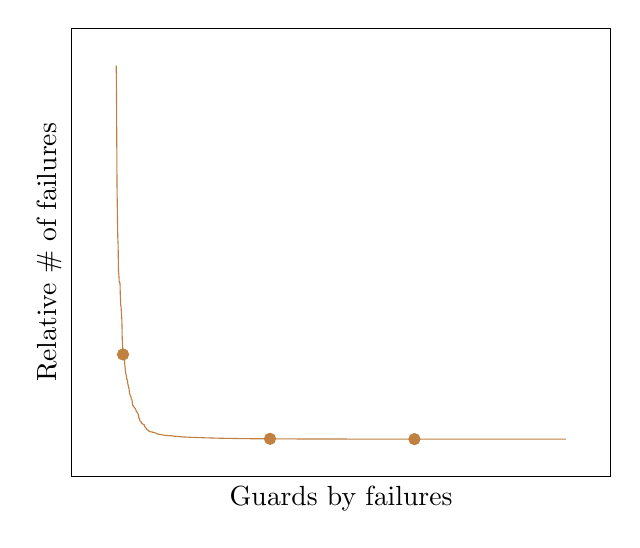
\begin{tikzpicture}
            \begin{axis}[
            xlabel= Guards by failures,
            ylabel=Relative \# of failures,
            xtick=\empty,
            ytick=\empty,
            ]
                
\addplot[brown,mark=none] coordinates {
(0.000000,1.000000) (0.000834,0.872400) (0.001668,0.683224) (0.002502,0.608314) (0.003336,0.542330) (0.004170,0.519721) (0.005004,0.447508) (0.005838,0.440065) (0.006672,0.420670) (0.007506,0.418862) (0.008340,0.418009) (0.009174,0.379519) (0.010008,0.357223) (0.010842,0.353534) (0.011676,0.333568) (0.012510,0.319704) (0.013344,0.268160) (0.014178,0.251065) (0.015013,0.226789) (0.015847,0.220089) (0.016681,0.215066) (0.017515,0.213903) (0.018349,0.213091) (0.019183,0.197153) (0.020017,0.187389) (0.020851,0.177430) (0.021685,0.173396) (0.022519,0.170787) (0.023353,0.160834) (0.024187,0.160045) (0.025021,0.157071) (0.025855,0.146612) (0.026689,0.144178) (0.027523,0.137699) (0.028357,0.136683) (0.029191,0.124833) (0.030025,0.121453) (0.030859,0.119189) (0.031693,0.115002) (0.032527,0.114249) (0.033361,0.107546) (0.034195,0.107268) (0.035029,0.104187) (0.035863,0.096624) (0.036697,0.089912) (0.037531,0.089585) (0.038365,0.087446) (0.039199,0.087298) (0.040033,0.084823) (0.040867,0.083414) (0.041701,0.083212) (0.042535,0.082227) (0.043369,0.079913) (0.044204,0.075734) (0.045038,0.073337) (0.045872,0.073039) (0.046706,0.072381) (0.047540,0.069693) (0.048374,0.067325) (0.049208,0.065996) (0.050042,0.057532) (0.050876,0.055707) (0.051710,0.055669) (0.052544,0.049083) (0.053378,0.048652) (0.054212,0.048015) (0.055046,0.045918) (0.055880,0.045234) (0.056714,0.042272) (0.057548,0.041798) (0.058382,0.040969) (0.059216,0.040163) (0.060050,0.040016) (0.060884,0.038778) (0.061718,0.038686) (0.062552,0.038456) (0.063386,0.033439) (0.064220,0.032381) (0.065054,0.031115) (0.065888,0.030103) (0.066722,0.029385) (0.067556,0.026654) (0.068390,0.025877) (0.069224,0.024467) (0.070058,0.024427) (0.070892,0.024134) (0.071726,0.024036) (0.072560,0.021379) (0.073394,0.020813) (0.074229,0.020166) (0.075063,0.020056) (0.075897,0.019981) (0.076731,0.019791) (0.077565,0.019672) (0.078399,0.019356) (0.079233,0.019269) (0.080067,0.019134) (0.080901,0.018119) (0.081735,0.017905) (0.082569,0.017878) (0.083403,0.017865) (0.084237,0.017769) (0.085071,0.017758) (0.085905,0.017065) (0.086739,0.016959) (0.087573,0.016686) (0.088407,0.015666) (0.089241,0.014908) (0.090075,0.014542) (0.090909,0.014518) (0.091743,0.014200) (0.092577,0.013865) (0.093411,0.013736) (0.094245,0.013273) (0.095079,0.013197) (0.095913,0.012997) (0.096747,0.012759) (0.097581,0.012642) (0.098415,0.012344) (0.099249,0.012031) (0.100083,0.011973) (0.100917,0.011805) (0.101751,0.011594) (0.102585,0.011387) (0.103420,0.011332) (0.104254,0.011246) (0.105088,0.010925) (0.105922,0.010566) (0.106756,0.010269) (0.107590,0.010235) (0.108424,0.010220) (0.109258,0.010135) (0.110092,0.010071) (0.110926,0.010048) (0.111760,0.010002) (0.112594,0.009762) (0.113428,0.009756) (0.114262,0.009751) (0.115096,0.009730) (0.115930,0.009551) (0.116764,0.009536) (0.117598,0.009404) (0.118432,0.009399) (0.119266,0.009298) (0.120100,0.009263) (0.120934,0.009245) (0.121768,0.009137) (0.122602,0.009120) (0.123436,0.009097) (0.124270,0.008816) (0.125104,0.008646) (0.125938,0.008484) (0.126772,0.008405) (0.127606,0.008149) (0.128440,0.008032) (0.129274,0.007872) (0.130108,0.007866) (0.130942,0.007823) (0.131776,0.007801) (0.132611,0.007718) (0.133445,0.007481) (0.134279,0.007373) (0.135113,0.007345) (0.135947,0.007296) (0.136781,0.007269) (0.137615,0.007233) (0.138449,0.006991) (0.139283,0.006905) (0.140117,0.006795) (0.140951,0.006738) (0.141785,0.006708) (0.142619,0.006551) (0.143453,0.006510) (0.144287,0.006435) (0.145121,0.006361) (0.145955,0.006238) (0.146789,0.006134) (0.147623,0.006027) (0.148457,0.005991) (0.149291,0.005921) (0.150125,0.005852) (0.150959,0.005852) (0.151793,0.005823) (0.152627,0.005794) (0.153461,0.005787) (0.154295,0.005746) (0.155129,0.005672) (0.155963,0.005619) (0.156797,0.005612) (0.157631,0.005557) (0.158465,0.005495) (0.159299,0.005495) (0.160133,0.005422) (0.160967,0.005324) (0.161802,0.005217) (0.162636,0.005196) (0.163470,0.005167) (0.164304,0.005107) (0.165138,0.005012) (0.165972,0.004999) (0.166806,0.004985) (0.167640,0.004981) (0.168474,0.004936) (0.169308,0.004912) (0.170142,0.004836) (0.170976,0.004822) (0.171810,0.004755) (0.172644,0.004692) (0.173478,0.004687) (0.174312,0.004667) (0.175146,0.004605) (0.175980,0.004546) (0.176814,0.004523) (0.177648,0.004518) (0.178482,0.004512) (0.179316,0.004447) (0.180150,0.004427) (0.180984,0.004408) (0.181818,0.004401) (0.182652,0.004336) (0.183486,0.004326) (0.184320,0.004255) (0.185154,0.004163) (0.185988,0.004152) (0.186822,0.004150) (0.187656,0.004132) (0.188490,0.004125) (0.189324,0.003972) (0.190158,0.003971) (0.190992,0.003942) (0.191827,0.003842) (0.192661,0.003797) (0.193495,0.003710) (0.194329,0.003703) (0.195163,0.003684) (0.195997,0.003626) (0.196831,0.003620) (0.197665,0.003576) (0.198499,0.003526) (0.199333,0.003451) (0.200167,0.003447) (0.201001,0.003402) (0.201835,0.003390) (0.202669,0.003364) (0.203503,0.003361) (0.204337,0.003356) (0.205171,0.003350) (0.206005,0.003341) (0.206839,0.003321) (0.207673,0.003278) (0.208507,0.003246) (0.209341,0.003239) (0.210175,0.003219) (0.211009,0.003208) (0.211843,0.003129) (0.212677,0.003123) (0.213511,0.003073) (0.214345,0.003063) (0.215179,0.003053) (0.216013,0.003053) (0.216847,0.003026) (0.217681,0.003007) (0.218515,0.002989) (0.219349,0.002929) (0.220183,0.002915) (0.221018,0.002913) (0.221852,0.002890) (0.222686,0.002861) (0.223520,0.002845) (0.224354,0.002804) (0.225188,0.002783) (0.226022,0.002781) (0.226856,0.002694) (0.227690,0.002669) (0.228524,0.002631) (0.229358,0.002579) (0.230192,0.002578) (0.231026,0.002573) (0.231860,0.002566) (0.232694,0.002507) (0.233528,0.002487) (0.234362,0.002486) (0.235196,0.002416) (0.236030,0.002367) (0.236864,0.002347) (0.237698,0.002344) (0.238532,0.002338) (0.239366,0.002330) (0.240200,0.002318) (0.241034,0.002315) (0.241868,0.002308) (0.242702,0.002308) (0.243536,0.002292) (0.244370,0.002287) (0.245204,0.002283) (0.246038,0.002264) (0.246872,0.002236) (0.247706,0.002227) (0.248540,0.002185) (0.249374,0.002173) (0.250209,0.002169) (0.251043,0.002135) (0.251877,0.002109) (0.252711,0.002039) (0.253545,0.002031) (0.254379,0.001987) (0.255213,0.001970) (0.256047,0.001966) (0.256881,0.001936) (0.257715,0.001908) (0.258549,0.001908) (0.259383,0.001893) (0.260217,0.001886) (0.261051,0.001882) (0.261885,0.001827) (0.262719,0.001827) (0.263553,0.001817) (0.264387,0.001797) (0.265221,0.001749) (0.266055,0.001742) (0.266889,0.001739) (0.267723,0.001727) (0.268557,0.001704) (0.269391,0.001700) (0.270225,0.001691) (0.271059,0.001690) (0.271893,0.001653) (0.272727,0.001600) (0.273561,0.001595) (0.274395,0.001555) (0.275229,0.001547) (0.276063,0.001546) (0.276897,0.001519) (0.277731,0.001513) (0.278565,0.001510) (0.279399,0.001505) (0.280234,0.001474) (0.281068,0.001468) (0.281902,0.001459) (0.282736,0.001458) (0.283570,0.001432) (0.284404,0.001410) (0.285238,0.001407) (0.286072,0.001401) (0.286906,0.001396) (0.287740,0.001391) (0.288574,0.001376) (0.289408,0.001372) (0.290242,0.001369) (0.291076,0.001345) (0.291910,0.001344) (0.292744,0.001318) (0.293578,0.001299) (0.294412,0.001295) (0.295246,0.001287) (0.296080,0.001285) (0.296914,0.001284) (0.297748,0.001270) (0.298582,0.001265) (0.299416,0.001253) (0.300250,0.001235) (0.301084,0.001233) (0.301918,0.001224) (0.302752,0.001222) (0.303586,0.001219) (0.304420,0.001209) (0.305254,0.001202) (0.306088,0.001191) (0.306922,0.001180) (0.307756,0.001173) (0.308590,0.001170) (0.309425,0.001167) (0.310259,0.001154) (0.311093,0.001147) (0.311927,0.001143) (0.312761,0.001130) (0.313595,0.001126) (0.314429,0.001124) (0.315263,0.001116) (0.316097,0.001115) (0.316931,0.001099) (0.317765,0.001088) (0.318599,0.001088) (0.319433,0.001082) (0.320267,0.001074) (0.321101,0.001071) (0.321935,0.001070) (0.322769,0.001066) (0.323603,0.001062) (0.324437,0.001047) (0.325271,0.001043) (0.326105,0.001041) (0.326939,0.001040) (0.327773,0.001038) (0.328607,0.001027) (0.329441,0.001025) (0.330275,0.001016) (0.331109,0.001016) (0.331943,0.000996) (0.332777,0.000992) (0.333611,0.000985) (0.334445,0.000979) (0.335279,0.000978) (0.336113,0.000978) (0.336947,0.000957) (0.337781,0.000953) (0.338616,0.000951) (0.339450,0.000947) (0.340284,0.000944) (0.341118,0.000939) (0.341952,0.000932) (0.342786,0.000930) (0.343620,0.000930) (0.344454,0.000928) (0.345288,0.000915) (0.346122,0.000914) (0.346956,0.000914) (0.347790,0.000911) (0.348624,0.000910) (0.349458,0.000908) (0.350292,0.000904) (0.351126,0.000895) (0.351960,0.000890) (0.352794,0.000887) (0.353628,0.000884) (0.354462,0.000879) (0.355296,0.000861) (0.356130,0.000861) (0.356964,0.000826) (0.357798,0.000814) (0.358632,0.000808) (0.359466,0.000800) (0.360300,0.000797) (0.361134,0.000796) (0.361968,0.000782) (0.362802,0.000779) (0.363636,0.000778) (0.364470,0.000777) (0.365304,0.000777) (0.366138,0.000775) (0.366972,0.000767) (0.367807,0.000764) (0.368641,0.000761) (0.369475,0.000758) (0.370309,0.000753) (0.371143,0.000753) (0.371977,0.000751) (0.372811,0.000738) (0.373645,0.000718) (0.374479,0.000718) (0.375313,0.000710) (0.376147,0.000709) (0.376981,0.000707) (0.377815,0.000701) (0.378649,0.000699) (0.379483,0.000694) (0.380317,0.000694) (0.381151,0.000688) (0.381985,0.000686) (0.382819,0.000683) (0.383653,0.000681) (0.384487,0.000665) (0.385321,0.000664) (0.386155,0.000660) (0.386989,0.000659) (0.387823,0.000657) (0.388657,0.000657) (0.389491,0.000655) (0.390325,0.000654) (0.391159,0.000647) (0.391993,0.000645) (0.392827,0.000644) (0.393661,0.000643) (0.394495,0.000642) (0.395329,0.000640) (0.396163,0.000639) (0.396997,0.000637) (0.397832,0.000634) (0.398666,0.000630) (0.399500,0.000614) (0.400334,0.000613) (0.401168,0.000607) (0.402002,0.000604) (0.402836,0.000603) (0.403670,0.000602) (0.404504,0.000602) (0.405338,0.000598) (0.406172,0.000597) (0.407006,0.000592) (0.407840,0.000588) (0.408674,0.000576) (0.409508,0.000572) (0.410342,0.000570) (0.411176,0.000570) (0.412010,0.000567) (0.412844,0.000567) (0.413678,0.000566) (0.414512,0.000564) (0.415346,0.000563) (0.416180,0.000554) (0.417014,0.000550) (0.417848,0.000548) (0.418682,0.000547) (0.419516,0.000547) (0.420350,0.000546) (0.421184,0.000542) (0.422018,0.000542) (0.422852,0.000535) (0.423686,0.000529) (0.424520,0.000518) (0.425354,0.000516) (0.426188,0.000515) (0.427023,0.000513) (0.427857,0.000512) (0.428691,0.000511) (0.429525,0.000503) (0.430359,0.000503) (0.431193,0.000503) (0.432027,0.000499) (0.432861,0.000497) (0.433695,0.000497) (0.434529,0.000495) (0.435363,0.000495) (0.436197,0.000494) (0.437031,0.000494) (0.437865,0.000492) (0.438699,0.000491) (0.439533,0.000490) (0.440367,0.000489) (0.441201,0.000488) (0.442035,0.000486) (0.442869,0.000484) (0.443703,0.000480) (0.444537,0.000479) (0.445371,0.000478) (0.446205,0.000471) (0.447039,0.000467) (0.447873,0.000466) (0.448707,0.000464) (0.449541,0.000460) (0.450375,0.000458) (0.451209,0.000456) (0.452043,0.000452) (0.452877,0.000451) (0.453711,0.000448) (0.454545,0.000446) (0.455379,0.000445) (0.456214,0.000444) (0.457048,0.000437) (0.457882,0.000436) (0.458716,0.000435) (0.459550,0.000431) (0.460384,0.000431) (0.461218,0.000430) (0.462052,0.000428) (0.462886,0.000428) (0.463720,0.000428) (0.464554,0.000427) (0.465388,0.000427) (0.466222,0.000422) (0.467056,0.000420) (0.467890,0.000415) (0.468724,0.000409) (0.469558,0.000408) (0.470392,0.000408) (0.471226,0.000406) (0.472060,0.000405) (0.472894,0.000404) (0.473728,0.000404) (0.474562,0.000402) (0.475396,0.000402) (0.476230,0.000402) (0.477064,0.000402) (0.477898,0.000399) (0.478732,0.000399) (0.479566,0.000398) (0.480400,0.000395) (0.481234,0.000395) (0.482068,0.000394) (0.482902,0.000390) (0.483736,0.000389) (0.484570,0.000387) (0.485405,0.000385) (0.486239,0.000383) (0.487073,0.000382) (0.487907,0.000381) (0.488741,0.000380) (0.489575,0.000380) (0.490409,0.000377) (0.491243,0.000375) (0.492077,0.000374) (0.492911,0.000373) (0.493745,0.000371) (0.494579,0.000370) (0.495413,0.000369) (0.496247,0.000368) (0.497081,0.000366) (0.497915,0.000364) (0.498749,0.000362) (0.499583,0.000362) (0.500417,0.000358) (0.501251,0.000354) (0.502085,0.000346) (0.502919,0.000345) (0.503753,0.000344) (0.504587,0.000343) (0.505421,0.000341) (0.506255,0.000340) (0.507089,0.000337) (0.507923,0.000337) (0.508757,0.000331) (0.509591,0.000328) (0.510425,0.000325) (0.511259,0.000323) (0.512093,0.000319) (0.512927,0.000319) (0.513761,0.000317) (0.514595,0.000315) (0.515430,0.000314) (0.516264,0.000313) (0.517098,0.000313) (0.517932,0.000312) (0.518766,0.000312) (0.519600,0.000311) (0.520434,0.000302) (0.521268,0.000300) (0.522102,0.000300) (0.522936,0.000295) (0.523770,0.000295) (0.524604,0.000295) (0.525438,0.000292) (0.526272,0.000290) (0.527106,0.000290) (0.527940,0.000288) (0.528774,0.000287) (0.529608,0.000285) (0.530442,0.000280) (0.531276,0.000278) (0.532110,0.000278) (0.532944,0.000278) (0.533778,0.000277) (0.534612,0.000276) (0.535446,0.000274) (0.536280,0.000273) (0.537114,0.000271) (0.537948,0.000271) (0.538782,0.000270) (0.539616,0.000266) (0.540450,0.000263) (0.541284,0.000260) (0.542118,0.000260) (0.542952,0.000258) (0.543786,0.000258) (0.544621,0.000256) (0.545455,0.000253) (0.546289,0.000252) (0.547123,0.000251) (0.547957,0.000249) (0.548791,0.000248) (0.549625,0.000248) (0.550459,0.000248) (0.551293,0.000246) (0.552127,0.000246) (0.552961,0.000244) (0.553795,0.000244) (0.554629,0.000242) (0.555463,0.000241) (0.556297,0.000240) (0.557131,0.000240) (0.557965,0.000239) (0.558799,0.000236) (0.559633,0.000236) (0.560467,0.000235) (0.561301,0.000234) (0.562135,0.000234) (0.562969,0.000234) (0.563803,0.000233) (0.564637,0.000233) (0.565471,0.000225) (0.566305,0.000223) (0.567139,0.000223) (0.567973,0.000220) (0.568807,0.000219) (0.569641,0.000218) (0.570475,0.000218) (0.571309,0.000217) (0.572143,0.000216) (0.572977,0.000213) (0.573812,0.000211) (0.574646,0.000207) (0.575480,0.000206) (0.576314,0.000206) (0.577148,0.000205) (0.577982,0.000205) (0.578816,0.000203) (0.579650,0.000203) (0.580484,0.000203) (0.581318,0.000203) (0.582152,0.000203) (0.582986,0.000201) (0.583820,0.000200) (0.584654,0.000200) (0.585488,0.000199) (0.586322,0.000199) (0.587156,0.000197) (0.587990,0.000194) (0.588824,0.000193) (0.589658,0.000191) (0.590492,0.000190) (0.591326,0.000190) (0.592160,0.000186) (0.592994,0.000186) (0.593828,0.000181) (0.594662,0.000178) (0.595496,0.000175) (0.596330,0.000174) (0.597164,0.000173) (0.597998,0.000173) (0.598832,0.000172) (0.599666,0.000171) (0.600500,0.000171) (0.601334,0.000170) (0.602168,0.000170) (0.603003,0.000169) (0.603837,0.000166) (0.604671,0.000165) (0.605505,0.000165) (0.606339,0.000165) (0.607173,0.000164) (0.608007,0.000163) (0.608841,0.000162) (0.609675,0.000162) (0.610509,0.000162) (0.611343,0.000162) (0.612177,0.000161) (0.613011,0.000161) (0.613845,0.000159) (0.614679,0.000158) (0.615513,0.000158) (0.616347,0.000157) (0.617181,0.000156) (0.618015,0.000155) (0.618849,0.000155) (0.619683,0.000152) (0.620517,0.000152) (0.621351,0.000151) (0.622185,0.000151) (0.623019,0.000149) (0.623853,0.000149) (0.624687,0.000148) (0.625521,0.000147) (0.626355,0.000147) (0.627189,0.000146) (0.628023,0.000146) (0.628857,0.000146) (0.629691,0.000146) (0.630525,0.000145) (0.631359,0.000145) (0.632193,0.000144) (0.633028,0.000144) (0.633862,0.000144) (0.634696,0.000144) (0.635530,0.000143) (0.636364,0.000142) (0.637198,0.000142) (0.638032,0.000142) (0.638866,0.000142) (0.639700,0.000141) (0.640534,0.000140) (0.641368,0.000139) (0.642202,0.000137) (0.643036,0.000137) (0.643870,0.000133) (0.644704,0.000131) (0.645538,0.000131) (0.646372,0.000129) (0.647206,0.000129) (0.648040,0.000129) (0.648874,0.000128) (0.649708,0.000128) (0.650542,0.000127) (0.651376,0.000124) (0.652210,0.000123) (0.653044,0.000119) (0.653878,0.000117) (0.654712,0.000117) (0.655546,0.000117) (0.656380,0.000115) (0.657214,0.000114) (0.658048,0.000114) (0.658882,0.000114) (0.659716,0.000113) (0.660550,0.000112) (0.661384,0.000111) (0.662219,0.000111) (0.663053,0.000111) (0.663887,0.000111) (0.664721,0.000110) (0.665555,0.000110) (0.666389,0.000109) (0.667223,0.000108) (0.668057,0.000108) (0.668891,0.000107) (0.669725,0.000105) (0.670559,0.000105) (0.671393,0.000105) (0.672227,0.000105) (0.673061,0.000105) (0.673895,0.000105) (0.674729,0.000105) (0.675563,0.000104) (0.676397,0.000104) (0.677231,0.000103) (0.678065,0.000102) (0.678899,0.000101) (0.679733,0.000101) (0.680567,0.000100) (0.681401,0.000100) (0.682235,0.000100) (0.683069,0.000099) (0.683903,0.000099) (0.684737,0.000098) (0.685571,0.000098) (0.686405,0.000098) (0.687239,0.000097) (0.688073,0.000094) (0.688907,0.000094) (0.689741,0.000092) (0.690575,0.000092) (0.691410,0.000091) (0.692244,0.000089) (0.693078,0.000089) (0.693912,0.000087) (0.694746,0.000087) (0.695580,0.000087) (0.696414,0.000086) (0.697248,0.000086) (0.698082,0.000086) (0.698916,0.000085) (0.699750,0.000085) (0.700584,0.000085) (0.701418,0.000085) (0.702252,0.000084) (0.703086,0.000084) (0.703920,0.000083) (0.704754,0.000083) (0.705588,0.000082) (0.706422,0.000081) (0.707256,0.000080) (0.708090,0.000080) (0.708924,0.000080) (0.709758,0.000079) (0.710592,0.000079) (0.711426,0.000078) (0.712260,0.000078) (0.713094,0.000077) (0.713928,0.000076) (0.714762,0.000076) (0.715596,0.000076) (0.716430,0.000075) (0.717264,0.000075) (0.718098,0.000072) (0.718932,0.000071) (0.719766,0.000071) (0.720601,0.000070) (0.721435,0.000070) (0.722269,0.000070) (0.723103,0.000070) (0.723937,0.000070) (0.724771,0.000070) (0.725605,0.000069) (0.726439,0.000068) (0.727273,0.000068) (0.728107,0.000068) (0.728941,0.000067) (0.729775,0.000067) (0.730609,0.000067) (0.731443,0.000067) (0.732277,0.000066) (0.733111,0.000066) (0.733945,0.000065) (0.734779,0.000065) (0.735613,0.000065) (0.736447,0.000065) (0.737281,0.000064) (0.738115,0.000064) (0.738949,0.000063) (0.739783,0.000063) (0.740617,0.000063) (0.741451,0.000062) (0.742285,0.000062) (0.743119,0.000060) (0.743953,0.000060) (0.744787,0.000059) (0.745621,0.000059) (0.746455,0.000059) (0.747289,0.000059) (0.748123,0.000058) (0.748957,0.000058) (0.749791,0.000057) (0.750626,0.000057) (0.751460,0.000057) (0.752294,0.000057) (0.753128,0.000057) (0.753962,0.000057) (0.754796,0.000057) (0.755630,0.000057) (0.756464,0.000057) (0.757298,0.000057) (0.758132,0.000057) (0.758966,0.000057) (0.759800,0.000057) (0.760634,0.000057) (0.761468,0.000057) (0.762302,0.000057) (0.763136,0.000056) (0.763970,0.000056) (0.764804,0.000055) (0.765638,0.000055) (0.766472,0.000055) (0.767306,0.000055) (0.768140,0.000055) (0.768974,0.000055) (0.769808,0.000054) (0.770642,0.000054) (0.771476,0.000054) (0.772310,0.000054) (0.773144,0.000054) (0.773978,0.000053) (0.774812,0.000053) (0.775646,0.000053) (0.776480,0.000053) (0.777314,0.000053) (0.778148,0.000053) (0.778982,0.000053) (0.779817,0.000052) (0.780651,0.000052) (0.781485,0.000052) (0.782319,0.000052) (0.783153,0.000052) (0.783987,0.000052) (0.784821,0.000052) (0.785655,0.000051) (0.786489,0.000051) (0.787323,0.000051) (0.788157,0.000051) (0.788991,0.000050) (0.789825,0.000050) (0.790659,0.000050) (0.791493,0.000049) (0.792327,0.000049) (0.793161,0.000049) (0.793995,0.000049) (0.794829,0.000049) (0.795663,0.000049) (0.796497,0.000049) (0.797331,0.000047) (0.798165,0.000047) (0.798999,0.000047) (0.799833,0.000047) (0.800667,0.000046) (0.801501,0.000046) (0.802335,0.000046) (0.803169,0.000046) (0.804003,0.000045) (0.804837,0.000045) (0.805671,0.000044) (0.806505,0.000044) (0.807339,0.000043) (0.808173,0.000043) (0.809008,0.000043) (0.809842,0.000043) (0.810676,0.000042) (0.811510,0.000042) (0.812344,0.000041) (0.813178,0.000041) (0.814012,0.000041) (0.814846,0.000041) (0.815680,0.000040) (0.816514,0.000040) (0.817348,0.000038) (0.818182,0.000038) (0.819016,0.000038) (0.819850,0.000037) (0.820684,0.000037) (0.821518,0.000037) (0.822352,0.000037) (0.823186,0.000037) (0.824020,0.000036) (0.824854,0.000036) (0.825688,0.000035) (0.826522,0.000035) (0.827356,0.000035) (0.828190,0.000035) (0.829024,0.000034) (0.829858,0.000034) (0.830692,0.000033) (0.831526,0.000033) (0.832360,0.000033) (0.833194,0.000033) (0.834028,0.000032) (0.834862,0.000032) (0.835696,0.000031) (0.836530,0.000031) (0.837364,0.000030) (0.838198,0.000030) (0.839033,0.000030) (0.839867,0.000030) (0.840701,0.000029) (0.841535,0.000029) (0.842369,0.000029) (0.843203,0.000029) (0.844037,0.000029) (0.844871,0.000028) (0.845705,0.000028) (0.846539,0.000028) (0.847373,0.000028) (0.848207,0.000028) (0.849041,0.000028) (0.849875,0.000028) (0.850709,0.000028) (0.851543,0.000028) (0.852377,0.000028) (0.853211,0.000028) (0.854045,0.000028) (0.854879,0.000028) (0.855713,0.000028) (0.856547,0.000028) (0.857381,0.000028) (0.858215,0.000028) (0.859049,0.000027) (0.859883,0.000027) (0.860717,0.000027) (0.861551,0.000027) (0.862385,0.000027) (0.863219,0.000027) (0.864053,0.000027) (0.864887,0.000027) (0.865721,0.000027) (0.866555,0.000027) (0.867389,0.000027) (0.868224,0.000027) (0.869058,0.000027) (0.869892,0.000026) (0.870726,0.000026) (0.871560,0.000026) (0.872394,0.000025) (0.873228,0.000025) (0.874062,0.000025) (0.874896,0.000025) (0.875730,0.000025) (0.876564,0.000025) (0.877398,0.000025) (0.878232,0.000025) (0.879066,0.000025) (0.879900,0.000025) (0.880734,0.000024) (0.881568,0.000024) (0.882402,0.000024) (0.883236,0.000024) (0.884070,0.000024) (0.884904,0.000024) (0.885738,0.000023) (0.886572,0.000023) (0.887406,0.000023) (0.888240,0.000023) (0.889074,0.000023) (0.889908,0.000023) (0.890742,0.000022) (0.891576,0.000022) (0.892410,0.000022) (0.893244,0.000022) (0.894078,0.000022) (0.894912,0.000022) (0.895746,0.000022) (0.896580,0.000022) (0.897415,0.000021) (0.898249,0.000021) (0.899083,0.000021) (0.899917,0.000021) (0.900751,0.000021) (0.901585,0.000021) (0.902419,0.000021) (0.903253,0.000021) (0.904087,0.000021) (0.904921,0.000021) (0.905755,0.000021) (0.906589,0.000021) (0.907423,0.000021) (0.908257,0.000020) (0.909091,0.000020) (0.909925,0.000020) (0.910759,0.000020) (0.911593,0.000020) (0.912427,0.000020) (0.913261,0.000020) (0.914095,0.000019) (0.914929,0.000019) (0.915763,0.000019) (0.916597,0.000018) (0.917431,0.000018) (0.918265,0.000018) (0.919099,0.000017) (0.919933,0.000017) (0.920767,0.000017) (0.921601,0.000017) (0.922435,0.000017) (0.923269,0.000016) (0.924103,0.000016) (0.924937,0.000016) (0.925771,0.000016) (0.926606,0.000016) (0.927440,0.000016) (0.928274,0.000015) (0.929108,0.000015) (0.929942,0.000015) (0.930776,0.000015) (0.931610,0.000015) (0.932444,0.000015) (0.933278,0.000015) (0.934112,0.000015) (0.934946,0.000014) (0.935780,0.000014) (0.936614,0.000014) (0.937448,0.000014) (0.938282,0.000013) (0.939116,0.000013) (0.939950,0.000012) (0.940784,0.000012) (0.941618,0.000012) (0.942452,0.000012) (0.943286,0.000012) (0.944120,0.000012) (0.944954,0.000012) (0.945788,0.000012) (0.946622,0.000011) (0.947456,0.000011) (0.948290,0.000011) (0.949124,0.000011) (0.949958,0.000011) (0.950792,0.000011) (0.951626,0.000010) (0.952460,0.000010) (0.953294,0.000010) (0.954128,0.000010) (0.954962,0.000009) (0.955796,0.000009) (0.956631,0.000009) (0.957465,0.000009) (0.958299,0.000008) (0.959133,0.000008) (0.959967,0.000008) (0.960801,0.000008) (0.961635,0.000008) (0.962469,0.000008) (0.963303,0.000008) (0.964137,0.000008) (0.964971,0.000007) (0.965805,0.000007) (0.966639,0.000007) (0.967473,0.000007) (0.968307,0.000007) (0.969141,0.000007) (0.969975,0.000006) (0.970809,0.000006) (0.971643,0.000006) (0.972477,0.000005) (0.973311,0.000005) (0.974145,0.000004) (0.974979,0.000004) (0.975813,0.000004) (0.976647,0.000004) (0.977481,0.000004) (0.978315,0.000003) (0.979149,0.000003) (0.979983,0.000003) (0.980817,0.000003) (0.981651,0.000002) (0.982485,0.000002) (0.983319,0.000002) (0.984153,0.000002) (0.984987,0.000002) (0.985822,0.000002) (0.986656,0.000001) (0.987490,0.000001) (0.988324,0.000001) (0.989158,0.000001) (0.989992,0.000001) (0.990826,0.000001) (0.991660,0.000001) (0.992494,0.000001) (0.993328,0.000001) (0.994162,0.000001) (0.994996,0.000001) (0.995830,0.000001) (0.996664,0.000001) (0.997498,0.000001) (0.998332,0.000001) (0.999166,0.000001) (1.000000,0.000001)
};
\addplot[brown,only marks,mark=*] coordinates {(0.015013,0.226789) (0.341952,0.000932) (0.663053,0.000111)};
    
            \end{axis}
        \end{tikzpicture}
    \end{figure}
\end{frame}

%\section{Evaluation}

%as in paper
%fancy graphs
%something about execution speed
% <demo, if there is time>
\end{document}
